% $Id$
% !Mode:: "TeX:DE"    % Setting document mode and submode for WinEdt
% ............................................................................
%       P & P - V E R S C H L U E S S E L U N G S V E R F A H R E N
% ~~~~~~~~~~~~~~~~~~~~~~~~~~~~~~~~~~~~~~~~~~~~~~~~~~~~~~~~~~~~~~~~~~~~~~~~~~~~

\begin{refsegment}

\newpage
\hypertarget{Chapter_PaperandPencil}{}

\chapter{Papier- und Bleistift-Verschlüsselungsverfahren}
\label{Chapter_PaperandPencil}
\chaptermark{Papier und Bleistift}
(\hyperlink{author_Christine-Stoetzel}{Christine Stötzel}, Apr. 2004;
 Updates B.+C. Esslinger, Juni 2005;
 Updates: \hyperlink{author_Minh-Van-Nguyen}{Minh Van Nguyen} und
	  \hyperlink{author_Bernhard-Esslinger}{Bernhard Esslinger}, Nov. 2009, Juni 2010;
	  \hyperlink{author_Bernhard-Esslinger}{Bernhard Esslinger}, Mai 2013, Aug. 2016)
\index{Papier- und Bleistiftverfahren}
\index{Verschlüsselung!klassisch}
\index{Kryptographie!klassisch}

\begin{ctsquote}
Nur Wenige kann man glauben machen, dass es keine leichte Sache ist,
eine Geheimschrift zu erdenken, die sich der Untersuchung widersetzt.
Dennoch kann man rundheraus annehmen, dass menschlicher Scharfsinn
keine Chiffre erdenken kann, die menschlicher Scharfsinn nicht lösen kann.
%\caption{Edgar Allan Poe: A Few Words on Secret Writing, 1841}
\caption[Edgar Allan Poe]{Edgar Allan Poe: A Few Words on Secret Writing, 1841}
\index{Poe, Edgar Allan}
\end{ctsquote}

Das folgende Kapitel bietet einen recht vollständigen Überblick über Papier-
und Bleistiftverfahren.\footnote{%
Die Fußnoten dieses Kapitel zeigen, wie man diese
Verfahren mit den Offline-Programmen CrypTool~1 (\textbf{CT1})\index{CT1},
CrypTool~2 (\textbf{CT2})\index{CT2} und JCrypTool (\textbf{JCT})\index{JCT}
ausführen kann. Vergleiche dazu die Anhänge
\ref{s:appendix-menu-overview-CT1},
\ref{s:appendix-template-overview-CT2} und
\ref{s:appendix-function-overview-JCT}.\\

Viele der Verfahren lassen sich auch online im Browser durchführen, z.B. auf
der Seite von CrypTool-Online (\textbf{CTO}) (\url{http://www.cryptool-online.org})\index{CTO}.
Vergleiche dazu den Anhang \ref{s:appendix-function-overview-CTO} in diesem Buch.\\

Während die CrypTool-Webseiten und -Programme sowohl klassische und moderne Chiffren
anbieten, gibt es auch mehrere Seiten, die sich mit großer Detailtiefe auf klassische
Chiffren fokussieren -- diese stehen oft in Verbindung mit der American Cryptogram
Association (ACA) (\url{http://www.cryptogram.org/}).\\
Zum Beispiel \url{https://sites.google.com/site/bionspot/} und
\url{https://encode-decode.appspot.com/} von Bion\index{Bion}.\\
Eine attraktive neue Seite, um klassiche Chiffren auszuführen, ist von
Phil Pilcrow (\url{www.cryptoprograms.com}). Diese Seite enthält auch Beschreibungen
und Beispiele für jeden Verfahrenstyp. Sein FAQ vom 23. Juli 2016 sagt:
\glqq The site is designed for creating classical cipher types, not machine based
or modern ones but if you want another cipher type added let me know.\grqq \index{Pilcrow, Phil}\\

Außerdem enthält das letzte Unterkapitel (\ref{PaP_Sage_samples}) dieses Kapitels
zu einigen Verfahren Beispielcode für das Computer-Algebra-System \textbf{SageMath}\index{SageMath}.
   }
Unter diesem Begriff lassen sich alle Verfahren zusammenfassen, die Menschen von
Hand anwenden können, um Nachrichten zu ver- und entschlüsseln.
Besonders populär waren diese Verfahren für Geheimdienste (und
sind es immer noch), da ein Schreibblock und ein Stift -- im
Gegensatz zu elektronischen Hilfsmitteln -- vollkommen unverdächtig sind.

Die ersten Papier- und Bleistiftverfahren entstanden bereits vor rund
3000 Jahren, aber auch während des vergangenen Jahrhunderts kamen
noch zahlreiche neue Methoden hinzu. Bei allen Papier- und
Bleistiftverfahren handelt es sich um symmetrische
Verfahren\index{Verschlüsselung!symmetrisch}. Selbst in den
ältesten Verschlüsselungsmethoden steckten schon die
grundsätzlichen Konstruktionsprinzipien wie Transposition,
Substitution, Blockbildung und deren Kombination. Daher
lohnt es sich vor allem aus didaktischen Gesichtspunkten,
diese "`alten"' Verfahren genauer zu betrachten.

Erfolgreiche bzw. verbreiteter eingesetzte Verfahren mussten die gleichen
Merkmale erfüllen wie moderne Verfahren:
\begin{itemize}
\item Vollständige Beschreibung, klare Regeln, ja fast Standardisierung
      (inkl. der Sonderfälle, dem Padding, etc.).
\item Gute Balance zwischen Sicherheit und Benutzbarkeit
      (denn zu kompliziert zu bedienende Verfahren waren fehlerträchtig
      oder unangemessen langsam).
\end{itemize}



%------------------------------------------------------------------------------
\newpage
\section{Transpositionsverfahren}
\label{PaP_transposition_ciphers}
\index{Transposition}

Bei der Verschlüsselung durch Transposition\index{Transposition}
bleiben die ursprünglichen Zeichen der Nachricht erhalten,
nur ihre Anordnung wird geändert (Transposition =
Vertauschung).\footnote{%
Manchmal wird auch der Begriff Permutation\index{Permutation} verwendet, um zu
beschreiben, wie Buchstaben, Buchstabengruppen oder Spalten des Klartextes
vertauscht werden, z.B. in der Form $(1, 2, 3, 4, 5)
\Leftrightarrow (3, 4, 2, 1, 5)$.
}

%------------------------------------------------------------------------------
\subsection{Einführende Beispiele}
\label{introsamplesTranspositionCiphers}  %be_2006 so ist es gut.

\begin{itemize}

\item \textbf{Gartenzaun-Chiffre}\footnote{%
   Dieses Verfahren kann direkt in CT1\index{CT1} mit dem Menüpunkt
   \textbf{Ver-/Entschlüsseln \textbackslash{} Symmetrisch (klassisch)
   \textbackslash{} Skytale / Gartenzaun} abgebildet werden.
   Man kann diese Methode auch simulieren über den Menüeintrag
   \textbf{Ver-/Entschlüsseln \textbackslash{} Symmetrisch (klassisch)
   \textbackslash{} Permutation}:
   Für einen Gartenzaun mit 2 Zeilen gibt man als Schlüssel
   \glqq B,A\grqq~ein und lässt ansonsten die Standardeinstellungen (nur 1
   Permutation, in der man zeilenweise ein- und spaltenweise ausliest).
   Mit dem Schlüssel "`A,B"' würde man das Zick-zack-Muster unten so
   beginnen, dass der erste Buchstabe in der ersten statt in der zweiten Zeile
   steht.}
   \cite{Singh2001}\index{Gartenzaun-Verschlüsselung}:
                        % Kein Blank VOR "\index", sonst ist der
                        % Doppelpunkt nicht direkt nach dem Fussnotenindex.
   Die Buchstaben des Klartextes werden abwechselnd in zwei (oder mehr)
   Zeilen geschrieben, so dass ein Zickzack-Muster entsteht.
   Dann werden die Zeichen zeilenweise nacheinander gelesen.\\
   Dieses Verfahren ist eher eine Kinderverschlüsselung.

   Siehe Tabelle \ref{PaP_RailFence_table-reference}.

   Klartext\footnote{%
     Konvention\index{Konvention}: Wenn das Alphabet nur die 26 Buchstaben
     verwendet, schreiben wir im Folgenden den Klartext in Kleinbuchstaben
     und den Geheimtext in Großbuchstaben.
   }:
   ein beispiel zur transposition

   \begin{table}[ht]
   \begin{center}
   \begin{tabular}{r@{\:}r@{\:}r@{\:}r@{\:}r@{\:}r@{\:}r@{\:}r@{\:}r@{\:}
                r@{\:}r@{\:}r@{\:}r@{\:}r@{\:}r@{\:}r@{\:}r@{\:}r@{\:}
                r@{\:}r@{\:}r@{\:}r@{\:}r@{\:}r@{\:}r@{\:}r@{\:}r@{\:}}
	  & i &   & b &   & i &   & p &   & e &   & z &   & r &   &
            r &   & n &   & p &   & s &   & t &   & o &   \\
	e &   & n &   & e &   & s &   & i &   & l &   & u &   & t &
          & a &   & s &   & o &   & i &   & i &   & n
   \end{tabular}
   \caption{Gartenzaun-Verschlüsselung}
   \label{PaP_RailFence_table-reference}
   \end{center}
   \end{table}

   Geheimtext\footnote{Die Buchstaben des Klartextes sind hier -- wie
   historisch üblich -- in 5-er Blöcken gruppiert. Man könnte o.E.d.A.
   auch eine andere (konstante) Blocklänge oder gar keine Trennung durch
   Leerzeichen wählen.}%
   : IBIPE ZRRNP STOEN ESILU TASOI IN\\


\item \textbf{Skytale von Sparta}\footnote{%
    Dieses Verfahren kann direkt in CT1\index{CT1} mit dem Menüpunkt
    \textbf{Ver-/Entschlüsseln \textbackslash{} Symmetrisch (klassisch)
    \textbackslash{} Skytale / Gartenzaun} abgebildet werden.
    Da dieses Verschlüsselungsverfahrens ein Spezialfall der einfachen
    Spaltentransposition ist, kann man es in CT1\index{CT1} auch
    über den Menüeintrag \textbf{Ver-/Entschlüsseln \textbackslash{}
    Symmetrisch (klassisch) \textbackslash{} Permutation} simulieren: Für die
    Skytale braucht man in der Dialogbox nur die erste Permutation. Darin gibt
    man bei z.B. 4 Kanten als Schlüssel  "`1,2,3,4"'  ein. Dies wäre so, als
    würde man den Text in 4-er Blöcken waagrecht in eine Tabelle schreiben und
    senkrecht auslesen.
    Weil der Schlüssel aufsteigend geordnet ist, bezeichnet man die Skytale
    auch als identische Permutation. Und weil das Schreiben und Auslesen nur
    einmal durchgeführt wird, als einfache (und nicht als doppelte) Permutation.\\
    In CT2\index{CT2} findet sich die Skytale bei den Vorlagen unter
    \textbf{Kryptographie \textbackslash{} Klassisch}.
   }
   \cite{Singh2001}\index{Skytale}%
   :
   Dieses Verfahren wurde wahrscheinlich das erste Mal um 600 v.Chr.
   benutzt und es wurde von dem griechischen Schriftsteller und Philosophen
   Plutarch (50-120 v.Chr.) zuerst beschrieben.\\
   Um einen Holzstab wird ein Streifen Papier o.ä. gewickelt. Dann wird
   darauf zeilenweise der Klartext geschrieben. Nach dem Abwickeln steht
   auf dem Streifen der Geheimtext. Zum Entschlüsseln braucht der Empfänger
   einen zuvor verabredeten gleich großen Holzstab mit gleich vielen Kanten.


\item \textbf{Schablonen-Chiffre} \cite{Goebel2014}: Sender und Empfänger
   benutzen die gleiche Schablone. In deren Löcher werden zeilenweise die
   Klartextzeichen geschrieben, die dann spaltenweise ausgelesen werden.
   Bleibt Klartext übrig, wird der Vorgang wiederholt, unter Umständen
   mit einer anderen Ausrichtung der Schablone.\footnote{%
   Dieses Verfahren kann man nicht durch eine einfache Spaltentransposition
   darstellen.}


   \hypertarget{turning-grille-cipher}{}   % References in movies.text
\item \textbf{Fleißner-Schablone} \cite{Savard1999}% verhindert, dass Blank vor ":"
   \index{Fleißner-Schablone}:
   Die Fleißner-Schablone wurde im Ersten Weltkrieg von deutschen Soldaten
   benutzt.\footnote{%
      Erfunden wurde die Fleißner-Schablone bereits 1881 von Eduard Fleißner
      von Wostrowitz.\\
      Eine gute Visualisierung findet sich unter www.turning-grille.com.\\
      In JCT\index{JCT} findet man es in der Standard-Perspektive
      über den Menüeintrag \textbf{Visualisierungen \textbackslash{} Grille}.
   }
   Ein quadratisches Gitter dient als Schablone, wobei ein Viertel der
   Felder Löcher hat. Der erste Teil des Klartextes wird zeichenweise
   durch die Löcher auf ein Blatt Papier geschrieben, dann wird die
   Schablone um 90 Grad gedreht, und der zweite Teil des Textes wird
   auf das Papier geschrieben, usw. Die Kunst besteht in der richtigen
   Wahl der Löcher: Kein Feld auf dem Papier darf frei bleiben, es
   darf aber auch keines doppelt beschriftet werden. Der Geheimtext
   wird zeilenweise ausgelesen.

   In die Beispiel-Fleißner-Schablone in Tabelle \ref{PaP_88Fleissner_table-reference}
   können 4 Mal je 16 Zeichen des Klartextes auf ein Blatt geschrieben werden:
   \begin{table}[ht]
   \begin{center}
   \begin{tabular}{|cccc|cccc|}
   \hline 	
	O & - & - & - & - & O & - & - \\
	- & - & - & O & O & - & - & O \\
	- & - & - & O & - & - & O & - \\
	- & - & O & - & - & - & - & - \\
   \hline 	
	- & - & - & - & O & - & - & - \\
	O & - & O & - & - & - & O & - \\
	- & O & - & - & - & - & - & O \\
	- & - & - & O & O & - & - & - \\
   \hline
   \end{tabular}
   \caption{8x8-Fleißner-Schablone}
   \label{PaP_88Fleissner_table-reference}
   \end{center}
   \end{table}

\end{itemize}


%------------------------------------------------------------------------------
\subsection[Spalten- und Zeilentranspositionsverfahren]
    {Spalten- und Zeilentranspositionsverfahren\footnotemark}
    \footnotetext{%
Die meisten der folgenden Verfahren können in CT1\index{CT1}
mit dem Menüpunkt \textbf{Ver-/Entschlüsseln \textbackslash{}
Symmetrisch (klassisch) \textbackslash{} Permutation} abgebildet werden.
% Todo: Add later same statement for CT2, if DCT is added there too. xxxxxxxxxxxxxxx
%       Some permutation analysis components are already there.
}

\begin{itemize}\sloppy

\item \textbf{Einfache Spaltentransposition} \cite{Savard1999}: Zunächst wird
   ein Schlüsselwort bestimmt, das über die Spalten eines Gitters geschrieben
   wird. Dann schreibt man den zu verschlüsseln"-den Text zeilenweise in dieses
   Gitter.
   Die Spalten werden entsprechend des Auftretens der Buchstaben des
   Schlüsselwortes im Alphabet durchnummeriert. In dieser Reihenfolge werden
   nun auch die Spalten ausgelesen und so der Geheimtext gebildet.\footnote{%
   Darstellung mit CT1: Eingabe eines Schlüssels für die erste Permutation,
   zeilenweise einlesen, spaltenweise permutieren und auslesen.\\
   In CT2\index{CT2} findet sich die Transposition bei den Vorlagen unter
   \textbf{Kryptographie \textbackslash{} Klassisch}. Diese Komponente visualisiert
   auch, wie der Text in die Matrix ein- und ausgelesen wird und wie die Spalten
   vertauscht werden.
   }

   Siehe Tabelle \ref{PaP_SimpColTransp_table-reference}.
	
   Klartext: ein beispiel zur transposition

   \begin{table}[ht]
   \begin{center}
   \begin{tabular}{|c|c|c|}
   \hline
	K & E & Y \\
   \hline
	e & i & n \\
	b & e & i \\
	s & p & i \\
	e & l & z \\
	u & r & t \\
	r & a & n \\
	s & p & o \\
	s & i & t \\
	i & o & n \\
   \hline
   \end{tabular}
   \caption{Einfache Spaltentransposition}
   \label{PaP_SimpColTransp_table-reference}
   \end{center}
   \end{table}

   Transpositionsschlüssel: K=2; E=1; Y=3. \\
   Geheimtext: IEPLR APIOE BSEUR SSINI IZTNO TN \\


\item \textbf{AMSCO-Chiffre} \cite{ACA2002}\index{AMSCO}: Die Klartextzeichen
   werden abwechselnd in Einer- und Zweiergruppen in ein Gitter geschrieben.
   Dann erfolgt eine Vertauschung der Spalten, anschließend das Auslesen.


\item \textbf{Doppelte Spaltentransposition (DST) / \glqq Doppelwürfel\grqq}
   \cite{Savard1999}\index{Doppelwürfel}:
   Die doppelte
   Spaltentransposition wurde häufig im Zweiten Weltkrieg und zu Zeiten des
   Kalten Krieges angewendet. Dabei werden zwei Spaltentranspositionen
   nacheinander durchgeführt, für die zweite Transposition wird ein neuer
   Schlüssel benutzt.\footnote{%
   Darstellung mit CT1: Eingabe eines Schlüssels für die 1. Permutation,
   zeilenweise einlesen, spaltenweise permutieren und auslesen.
   Eingabe eines (neuen) Schlüssels für die 2. Permutation, Ergebnis der
   1. Permutation zeilenweise einlesen, spaltenweise permutieren und
   auslesen.
   % Todo: Add later same statement for CT2, if DCT is added there too. xxxxxxxxxxxx
   }\\
   Werden zwei unterschiedliche und genügend lange Schlüssel (mindestens je 20
   Zeichen) verwendet, dann ist das auch für heutige Computer noch eine
   Herausforderung.\footnote{%
     In MTC3\index{MTC3} finden sich dazu Challenges, bspw.\\
     \url{http://www.mysterytwisterc3.org/de/challenges/level-x-kryptographie-challenges/doppelwuerfel} und\\
     \url{https://www.mysterytwisterc3.org/de/challenges/level-3-kryptographie-challenges/doppelwuerfel-reloaded-teil-1}
   }


\item \textbf{Spaltentransposition, General Luigi Sacco} \cite{Savard1999}: Die
   Spalten eines Gitters werden den Buchstaben des Schlüsselwortes
   entsprechend nummeriert. Der Klartext wird dann zeilenweise eingetragen,
   in der ersten Zeile bis zur Spalte mit der Nummer 1, in der zweiten Zeile
   bis zur Spalte mit der Nummer 2 usw. Das Auslesen erfolgt wiederum
   spaltenweise.

   Siehe Tabelle \ref{PaP_LuigiSacco_table-reference}.

   Klartext: ein beispiel zur transposition

   \begin{table}[ht]
   \begin{center}
   \begin{tabular}{|c|c|c|c|c|c|c|}
   \hline
	G & E & N & E & R & A & L\\
	4 & 2 & 6 & 3 & 7 & 1 & 5\\
   \hline
	e & i & n & b & e & i &  \\
	s & p &   &   &   &   &  \\
	i & e & l & z &   &   &  \\
	u &   &   &   &   &   &  \\
	r & t & r & a & n & s & p\\
	o & s & i &   &   &   &  \\
	t & i & o & n &   &   &  \\
   \hline
   \end{tabular}
   \caption{Spaltentransposition nach General Luigi Sacco}
   \label{PaP_LuigiSacco_table-reference}
   \end{center}
   \end{table}

   Geheimtext: ESIUR OTIPE TSINL RIOBZ ANENI SP\\


\item \textbf{Spaltentransposition, Französische Armee im Ersten Weltkrieg}
   \cite{Savard1999}:
   Nach Durch"-führung einer Spaltentransposition werden diagonale Reihen
   ausgelesen.


\item \textbf{Zeilentransposition} \cite{Savard1999}: Der Klartext wird in gleich
   lange Blöcke zerlegt, was auch mit Hilfe eines Gitters erfolgen kann. Dann
   wird die Reihenfolge der Buchstaben bzw. der Spalten vertauscht. Da das
   Auslesen zeilenweise erfolgt, wird nur jeweils innerhalb der Blöcke
   permutiert.\footnote{%
   Darstellung mit CT1: Eingabe eines Schlüssels für die 1. Permutation,
   zeilenweise einlesen, spaltenweise permutieren und zeilenweise auslesen.\\
   In CT2\index{CT2} findet sich die Transposition bei den Vorlagen unter
   \textbf{Kryptographie \textbackslash{} Klassisch}. Diese Komponente visualisiert
   auch die zeilenweise Transposition.
   }

\end{itemize}
% Ende \subsection{Spalten- und Zeilentranspositionsverfahren}



%------------------------------------------------------------------------------
\subsection{Weitere Transpositionsverfahren}

\begin{itemize}

\item \textbf{Geometrische Figuren} \cite{Goebel2014}: Einem bestimmten Muster
   folgend wird der Klartext in ein Gitter geschrieben (Schnecke, Rösselsprung
   o.ä.), einem zweiten Muster folgend wird der Geheimtext ausgelesen.

\item \textbf{Union Route Cipher} \cite{Goebel2014}: Die Union Route Cipher hat
   ihren Ursprung im Amerikanischen Bürgerkrieg. Nicht die Buchstaben einer
   Nachricht werden umsortiert, sondern die Wörter. Für besonders prägnante
   Namen und Bezeichnungen gibt es Code"-wörter, die zusammen mit den Routen
   in einem Codebuch festgehalten werden. Eine Route bestimmt die Größe des
   Gitters, in das der Klartext eingetragen wird und das Muster, nach dem der
   Geheimtext ausgelesen wird. Zusätzlich gibt es eine Anzahl von
   Füllwörtern.

\item \textbf{Nihilist-Transposition} \cite{ACA2002}%
   \index{Nihilist-Transposition}:
   Der Klartext wird in eine
   quadratische Matrix eingetragen, an deren Seiten jeweils der gleiche
   Schlüssel steht. Anhand dieses Schlüssels werden sowohl die Zeilen als
   auch die Spalten alphabetisch geordnet und der Inhalt der Matrix
   dementsprechend umsortiert. Der Geheimtext wird zeilenweise ausgelesen.

   Siehe Tabelle \ref{PaP_NihilistTransp_table-reference}.

   Klartext: ein beispiel zur transposition

   \begin{table}[ht]
   \begin{center}
   \begin{tabular}{|c|ccccc||cc|ccccc|}
   \hline
	  & K & A & T & Z & E &   &   & A & E & K & T & Z\\
   \hline
	K & e & i & n & b & e &   & A & s & e & i & p & i\\
	A & i & s & p & i & e &   & E & s & i & o & i & t\\
	T & l & z & u & r & t &   & K & i & e & e & n & b\\
	Z & r & a & n & s & p &   & T & z & t & l & u & r\\
	E & o & s & i & t & i &   & Z & a & p & r & n & s\\
   \hline
   \end{tabular}
   \caption[Nihilist-Transposition]{Nihilist-Transposition\footnotemark}
   \label{PaP_NihilistTransp_table-reference}
   \end{center}
   \end{table}

   Geheimtext: SEIPI SIOIT IEENB ZTLUR APRNS\\
   \footnotetext{%
   Der linke Block ist das Resultat nach dem Einlesen. Der rechte Block ist
   das Resultat nach dem Vertauschen von Zeilen und Spalten.}


\item \textbf{Cadenus-Chiffre} \cite{ACA2002}\index{Cadenus}:
   Hierbei handelt es sich um eine
   Spalten"-transposition, die zwei Schlüs"-sel"-worte benutzt.\\
   Das erste Schlüsselwort wird benutzt, um die Spalten zu vertauschen.\\
   Das zweite Schlüsselwort wird benutzt, um das Startzeichen jeder Spalte
   festzulegen: dieses zweite Schlüsselwort ist eine beliebige Permutation
   des benutzten Alphabets. Diese schreibt man links vor die erste Spalte.
   Jede Spalte wird dann vertikal so verschoben (wrap-around), dass sie mit dem
   Buchstaben beginnt, der in derjenigen Zeile, wo der Schlüsselbuchstabe des
   ersten Schlüsselwortes in dem zweiten Schlüsselwort zu finden ist.\\
   Der Geheimtext wird zeilenweise ausgelesen.

   Siehe Tabelle \ref{PaP_Cadenus-table-reference}.

   Klartext: ein laengeres beispiel zur transposition mit cadenus

   \begin{table}[ht]
   \begin{center}
   \begin{tabular}{|c|ccc|ccc|ccc|}
   \hline
	  & K & \textbf{E} & Y & \textbf{E} & K & Y & \textbf{E} & K & Y\\
   \hline
	A & e & i & n & i & e & n & \textbf{p} & r & n\\
	D & l & a & e & a & l & e & i & b & o\\
	X & n & g & e & g & n & e & o & s & t\\
	K & r & e & s & e & \textbf{r} & s & i & e & n\\
	C & b & e & i & e & b & i & a & u & t\\
	W & s & p & i & p & s & i & n & r & d\\
	N & e & l & z & l & e & z & i & s & u\\
	S & u & r & t & r & u & t & a & s & n\\
	Y & r & a & n & a & r & \textbf{n} & g & i & e\\
	\textbf{E} & s & \textbf{p} & o & \textbf{p} & s & o & e & m & e\\
	D & s & i & t & i & s & t & e & c & s\\
	T & i & o & n & o & i & n & p & e & i\\	
	U & m & i & t & i & m & t & l & s & i\\
	B & c & a & d & a & c & d & r & e & z\\
	R & e & n & u & n & e & u & a & l & t\\
	G & s & - & - & - & s & - & - & n & -\\
   \hline
   \end{tabular}
%be_2005: Fußnote zur Tabellenüberschrift wird nur angezeigt, wenn man das
%         \footnotetext-Statement nicht direkt hinter \caption{...} schreibt,
%         sondern außerhalb!
%\caption{Cadenus\footnotemark}
   \caption[Cadenus]{Cadenus-Chiffre\footnotemark}
   \label{PaP_Cadenus-table-reference}
   \end{center}
   \end{table}%  be_2005: Das % ist nötig: sonst ist "Geheimtext" etwas eingerückt.
           %           Noch besser: Man lässt das % weg und fügt dafür eine
           %           Leerzeile nach \end{table} ein, denn dann wird nicht
           %           mehr der "Geheimtext..." VOR die Tabelle gedruckt !!

   Geheimtext: PRNIB OOSTI ENAUT NRDIS UASNG IEEME ECSPE ILSIR EZALT N\\
   \footnotetext{%
   In dem zweiten Dreierblock sind diejenigen Zeichen fett, die nach
   der Anwendung des zweiten Schlüsselwortes oben im dritten Dreierblock
   stehen.}

\end{itemize}



%------------------------------------------------------------------------------
% \newpage
\clearpage
\section{Substitutionsverfahren}
\label{PaP_substitution_ciphers}
\index{Substitution}


%------------------------------------------------------------------------------
\subsection{Monoalphabetische Substitutionsverfahren}
Monoalphabetische Substitutionsverfahren\index{Substitution!monoalphabetisch}
ordnen jedem Klartextzeichen ein Geheimtextzeichen fest zu, d.h. diese
Zuordnung ist während des ganzen Verschlüsselungsprozesses dieselbe.
\label{monoalphabeticSubstitutionCiphers}

\begin{itemize}\sloppy

\item \textbf{Allgemeine monoalphabetische Substitution / Zufällige
   Buchstabenzuordnung\footnotemark}
   \footnotetext{%
    Dieses Verfahren kann in CT1\index{CT1} mit dem Menüpunkt
    \textbf{Ver-/Entschlüsseln \textbackslash{} Symmetrisch (klassisch) \textbackslash{}
    Substitution / Atbash} abgebildet werden.\\
    In CT2\index{CT2} finden sich diese Verfahren bei den Vorlagen unter
    \textbf{Kryptographie \textbackslash{} Klassisch}.
    Entsprechende Analyzer finden sich bei den Vorlagen unter
    \textbf{Kryptoanalyse \textbackslash{} Klassisch}.
   }
   \cite{Singh2001}: Die Substitution erfolgt aufgrund einer festgelegten
   Zuordnung der Einzelbuchstaben.

\item \textbf{Atbash-Chiffre\footnotemark}
   \footnotetext{%
   Dieses Verfahren kann in CT1\index{CT1} mit dem Menüpunkt
   \textbf{Ver-/Entschlüsseln \textbackslash{} Symmetrisch (klassisch) \textbackslash{}
   Substitution / Atbash} abgebildet werden.
   }
   \cite{Singh2001}\index{Atbash}: Der erste Buchstabe des Alphabets wird
   durch den letzten Buchstaben des Alphabets ersetzt, 	der zweite durch den
   vorletzten, usw.

\item \textbf{Verschiebe-Chiffre, z.B. Caesar}\footnote{In CT1\index{CT1}
   kann man dieses Verfahren an drei verschiedenen Stellen im Menü finden:\\
   - \textbf{Ver-/Entschlüsseln \textbackslash{} Symmetrisch (klassisch)
     \textbackslash{} Caesar / ROT13} \\
   - \textbf{Analyse \textbackslash{} Symmetrische Verschlüsselung (klassisch)
     \textbackslash{} Ciphertext only \textbackslash{} Caesar} \\
   - \textbf{Einzelverfahren \textbackslash{} Visualisierung von Algorithmen
     \textbackslash{} Caesar}.
   }
   \cite{Singh2001}\index{Caesar}\index{Verschiebechiffre}%
   : Klartext- und Geheimtextalphabet werden um eine bestimmte Anzahl von
   Zeichen gegeneinander verschoben.

   Klartext:\\ 	\texttt{bei der caesarchiffre wird um drei stellen verschoben}

   Geheimtext:\\ \texttt{EHL GHU FDHVDUFKLIIUH ZLUG XP GUHL VWHOOHQ YHUVFKREHQ}


\item \textbf{Affine Chiffre}\footnote{
   Mit SageMath sind dazu unter \ref{PaP_affine_cipher_sage-sample} einige Beispiele
   implementiert.}%
   \index{affine Chiffre}: Dies ist eine Verallgemeinerung
   der Verschiebechiffre. Jeder Klartext-Buchstabe wird erst durch einen anderen
   ersetzt und das Ergebnis wird dann mit der Verschiebechiffre verschlüsselt.
   Die Bezeichnung \glqq affine Chiffre\grqq~kommt daher, dass man die
   Ver- und Entschlüsselung als affine bzw. lineare Funktion beschreiben kann.


\item \textbf{Substitution mit Symbolen, z.B. Freimaurerchiffre}
   \cite{Singh2001}: Ein Buchstabe wird durch ein Symbol ersetzt.

\item \textbf{Varianten}: Füller, absichtliche Fehler \cite{Singh2001}.

\item \textbf{Nihilist-Substitution}\footnote{Eine Animation zu diesem
   Nihilist-Verfahren findet sich in CT1\index{CT1} unter dem Menüpunkt
     \textbf{Einzelverfahren \textbackslash{} Visualisierung von Algorithmen
     \textbackslash{} Nihilist}.\\
     In CT2\index{CT2} findet sich Nihilist bei den Vorlagen unter
     \textbf{Kryptographie \textbackslash{} Klassisch}.
   }
   \cite{ACA2002}\index{Nihilist-Substitution}: Das Alphabet wird in
   eine 5x5-Matrix eingetragen und bei der Verarbeitung wird jedem Klartextbuchstaben
   die aus Zeilen- und Spaltennummer gebildete Zahl zugeordnet.
   Dann wird ein Schlüsselwort gewählt und über eine zweite Tabelle geschrieben.
   In diese wird der Klartext zeilenweise eingetragen.
   Die Geheimtextzeichen sind die Summen aus den
   Zahlen des Klartextes und den Zahlen des Schlüsselwortes. Bei Zahlen
   zwischen 100 und 110 wird die führende "`1"' ignoriert, so dass jeder
   Buchstabe durch eine zweistellige Zahl repräsentiert wird.

   Siehe Tabelle \ref{Nihilist-substitution-table-reference}.
	
   Klartext: ein beispiel zur substitution

% \begin{minipage}  Das um die Table herum führt nur zu Tex-Fehlern!
% Hier nun um 2 Tabellen nur 1 TABLE: Table hat 2 Wirkungen:
%   a) sagt TeX, dass er es frei vertikal positionieren kann.
%   b) dass man eine Nummerierung erhält und einen Index erstellen kann.
   \begin{table}[ht]

   \begin{center}
   Matrix~~   % Text links vor eine Table und 2 Blanks dazu
   \begin{tabular}{|c|ccccc|}
   \hline 	
	  & 1 & 2 & 3 & 4 & 5\\
   \hline
	1 & S & C & H & L & U\\
	2 & E & A & B & D & F\\
	3 & G & I & K & M & N\\
	4 & O & P & Q & R & T\\
	5 & V & W & X & Y & Z\\
   \hline
   \end{tabular}
   \end{center}

   \begin{center}
   Tabelle~~
   \begin{tabular}{|ccc|}
   \hline 	
	K & E & Y\\
	(33) & (21) & (54)\\
   \hline
	e & i & n\\
	(54) & (53) & (89)\\
	b & e & i\\
	(56) & (42) & (86)\\
	s & p & i\\
	(44) & (63) & (86)\\
	e & l & z\\
	(54) & (35) & (109)\\
	u & r & s\\
	(48) & (65) & (65)\\
	u & b & s\\
	(48) & (44) & (65)\\
	t & i & t\\
	(78) & (53) & (99)\\
	u & t & i\\
	(48) & (66) & (86)\\
	o & n &   \\	
	(74) & (56)&   \\
   \hline
   \end{tabular}
   \caption{Nihilist-Substitution}
   \label{Nihilist-substitution-table-reference} %Ans Ende legen; analog bei figure!
   \end{center}

   \end{table}%
   % \end{minipage}  Verträgt sich nicht mit TABLE.
	
   Geheimtext:
   54 53 89 56 42~~~86 44 63 86 54~~~35 09 48 65 65
   48 44 65 78 53~~~99 48 66 86 74~~~56\\


\item \textbf{Codes} \cite{Singh2001}: Im Laufe der Geschichte wurden immer
   wieder Codebücher verwendet. In diesen Büchern wird jedem möglichen
   \textbf{Wort} eines Klartextes ein Codewort, ein Symbol oder eine Zahl
   zugeordnet.
   Voraussetzung für eine erfolgreiche geheime Kommunikation ist, dass
   Sender und Empfänger exakt das gleiche Codebuch besitzen und die
   Zuordnung der Codewörter zu den Klartextwörtern nicht offengelegt wird.

\item \textbf{Nomenklator} \cite{Singh2001}\index{Nomenklator}:
   Als Nomenklator werden Techniken bezeichnet, die ein Verschlüsselungsverfahren
   mit einem Codebuch kombinieren. Meist basiert das Verschlüsselungssystem auf
   einem Geheimtextalphabet, mit dem ein Großteil der Nachricht chiffriert
   (via Substitution) wird. Für besonders häufig auftretende oder
   geheim zu haltende Wörter existieren eine begrenzte Anzahl von Codewörtern.

\item \textbf{Landkarten-Chiffre} \cite{ThinkQuest1999}\index{Landkarten-Chiffre}:
   Diese Methode stellt eine Kombination aus
   Substitution und Steganographie\footnote{Statt eine Nachricht zu
   verschlüsseln, versucht man bei der reinen
   Steganographie\index{Steganographie}, die Existenz
   der Nachricht zu verbergen.} dar.
   Klartextzeichen werden durch Symbole ersetzt, diese werden nach bestimmten
   Regeln in Landkarten angeordnet.


\item \textbf{Straddling Checkerboard}
   \cite{Goebel2014}\index{Straddling Checkerboard}:
   Eine 3x10-Matrix wird
   mit den Buchstaben des Alphabets und zwei beliebigen Sonderzeichen oder
   Zahlen gefüllt, indem zunächst die voneinander verschiedenen Zeichen
   eines Schlüsselwortes und anschließend die restlichen Buchstaben des
   Alphabets eingefügt werden. Die Spalten der Matrix werden mit den Ziffern
   0 bis 9, die zweite und dritte Zeile der Matrix mit den Ziffern 1 und 2
   nummeriert. Jedes Zeichen des Geheimtextes wird durch die entsprechende
   Ziffer bzw. das entsprechende Ziffernpaar ersetzt. Da die 1 und die 2
   die ersten Ziffern der möglichen Ziffernkombinationen sind, werden
   sie nicht als einzelne Ziffern verwendet.

   Siehe Tabelle \ref{Straddling-Checkerboard-table-reference}.

   Klartext: substitution bedeutet ersetzung  % hiernach Leerzeile, nichts stattdessen
                                              % ein \\, sonst wird, wenn die Tabelle
                                              % später kommt, der Abstand doppelt.
                                              % Warum auch immer?!

   \begin{table}[ht]
   \begin{center}
   \begin{tabular}{|c|cccccccccc|}
   \hline
	  & 0 & 1 & 2 & 3 & 4 & 5 & 6 & 7 & 8 & 9\\
   \hline
	  & S & - & - & C & H & L & U & E & A & B\\
	1 & D & F & G & I & J & K & M & N & O & P\\
	2 & Q & R & T & V & W & X & Y & Z & . & /\\
   \hline
   \end{tabular}
   \caption{Straddling Checkerboard mit Passwort \glqq Schluessel\grqq}
   \label{Straddling-Checkerboard-table-reference}
   \end{center}
   \end{table}

   Geheimtext: 06902 21322 23221 31817 97107 62272 27210 72227 61712\\

   Auffällig ist die Häufigkeit der Ziffern 1 und 2,
   dies wird jedoch durch die folgende Variante behoben.\\


\item \textbf{Straddling Checkerboard, Variante} \cite{Goebel2014}%
   \index{Straddling Checkerboard}:
   Diese Form des Straddling Checkerboards wurde von sowjetischen Spionen
   im Zweiten Weltkrieg entwickelt. Angeblich haben auch Ernesto (Ch\'e)
   Guevara\index{Ch\'e Guevara} und Fidel Castro diese Chiffre zur geheimen
   Kommunikation benutzt.\footnote{%
     Zusätzlich benutzte Ch\'e Guevara für seine Kommunikation mit Fidel Castro
     auch ein One-Time-Pad\index{OTP}.\\
     Siehe Teil 3 aus der Artikelserie {\em RSA \& Co. in der Schule:
     Moderne Kryptologie, alte Mathematik, raffinierte Protokolle}:
     \cite{Witten1999}, S. 52.\index{RSA \& Co. in der Schule}
   }
   Das Alphabet wird in ein Gitter eingetragen (Spaltenanzahl = Länge des
   Schlüsselwortes), und es werden zwei beliebige Ziffern als "`reserviert"'
   festgelegt, die später die zweite und dritte Zeile einer
   3x10-Matrix bezeichnen (in unserem Bsp. 3 und 7). Nun wird das Gitter mit
   dem erzeugten Alphabet spaltenweise durchlaufen und Buchstaben zeilenweise
   in die Matrix übertragen:
   Die acht häufigsten Buchstaben (ENIRSATD für die deutsche Sprache)
   bekommen zur schnelleren Chiffrierung die Ziffern 0 bis 9 zugewiesen,
   dabei werden die reservierten Ziffern nicht vergeben. Die übrigen
   Buchstaben werden der Reihe nach in die Matrix eingetragen.
   Gegebenenfalls wird als zweite Stufe der Verschlüsselung zum Geheimtext
   noch eine beliebige Ziffernfolge addiert.

   Siehe Tabelle \ref{Straddling-Checkerboard-variant-table-reference}.

   Klartext: substitution bedeutet ersetzung

   \begin{table}[ht]

   \begin{center}
   Gitter~~
   \begin{tabular}{|c|c|c|c|c|c|}
   \hline 		
	\textbf{S} & C & H & L & U & \textbf{E}\\
   \hline
	\textbf{A} & B & \textbf{D} & F & G & \textbf{I}\\
   \hline
	J & K & M & \textbf{N} & O & P\\
   \hline
	Q & \textbf{R} & \textbf{T} & V & W & X\\
   \hline
	Y & Z & . & / &   &    \\
   \hline
   \end{tabular}
   \end{center}

   \begin{center}
   Matrix~~
   \begin{tabular}{|c|cccccccccc|}
   \hline 	
	  & 0 & 1 & 2 & 3 & 4 & 5 & 6 & 7 & 8 & 9\\
   \hline
	  & \textbf{S} & \textbf{A} & \textbf{R} & - & \textbf{D} & \textbf{T} & \textbf{N} & - & \textbf{E} & \textbf{I}\\
	3 & J & Q & Y & C & B & K & Z & H & M & .\\
	7 & L & F & V & / & U & G & O & W & P & X\\
   \hline
   \end{tabular}
   \caption{Variante des Straddling Checkerboards}
   \label{Straddling-Checkerboard-variant-table-reference}
   \end{center}

   \end{table}

   Geheimtext: 07434 05957 45976 63484 87458 58208 53674 675\\


   \begin{itemize}
      \item \textbf{Ch\'e Guevara-Chiffre}:
      Einen Spezialfall dieser Variante benutzte Ch\'e Guevara (mit einem
      zusätzlichen Substitutionsschritt und einem leicht modifizierten Checkerboard):
	 \begin{itemize}
	    \item Die sieben häufigsten Buchstaben im Spanischen werden auf
               die erste Zeile verteilt.
            \item Es werden vier statt drei Zeilen benutzt.
            \item Damit konnte man $10*4 - 4 = 36 $ verschiedene Zeichen
               verschlüsseln.\\
         \end{itemize}
   \end{itemize}



\item \textbf{Tri-Digital-Chiffre} \cite{ACA2002}:
   Aus einem Schlüssel"-wort der Länge 10 wird ein numerischer Schlüs"-sel
   gebildet, indem die Buchstaben entsprechend ihres Auftretens im Alphabet
   durchnummeriert werden. Dieser Schlüssel wird über ein Gitter mit zehn
   Spalten geschrieben. In dieses Gitter wird unter Verwendung eines
   Schlüsselwortes zeilenweise das Alphabet eingetragen, wobei die letzte
   Spalte frei bleibt. Die Klartextzeichen werden durch die Zahl über der
   entsprechenden Spalte substituiert, die Zahl über der freien Spalte dient
   als Trennzeichen zwischen den einzelnen Wörtern.\\


\item \textbf{Baconian-Chiffre} \cite{ACA2002}\index{Baconian Cipher}:
   Jedem Buchstaben des Alphabets und 6 Zahlen oder Sonderzeichen wird ein
   fünfstelliger Binärcode zugeordnet (zum Beispiel 00000 = A, 00001 = B,
   usw.). Die Zeichen der Nachricht werden entsprechend ersetzt. Nun benutzt
   man eine zweite, unverdächtige Nachricht, um darin den Geheimtext zu
   verbergen. Dies kann zum Beispiel durch Klein- und Großschreibung oder
   kursiv gesetzte Buchstaben geschehen: man schreibt z.B. alle Buchstaben
   in der unverdächtigen Nachricht groß, die unter einer \glqq 1\grqq~
   stehen. Insgesamt fällt das sicher auf.

   Siehe Tabelle \ref{Baconian-table-reference}.

   \begin{table}[ht]
   \begin{center}
   \begin{tabular}{|c|ccccc|}
   \hline
        Nachricht                &  H   &   I   &   L   &   F   &   E     \\
   \hline
	Geheimtext               & {\tt 00111} & {\tt 01000} & {\tt 01011} & {\tt 00101} & {\tt 00100}   \\
	Unverdächtige Nachricht & {\tt esist} & {\tt warmu} & {\tt nddie} & {\tt sonne} & {\tt scheint} \\
   \hline
	Baconian Cipher          & {\tt esIST} & {\tt wArmu} & {\tt nDdIE} & {\tt soNnE} & {\tt scHeint} \\
   \hline
   \end{tabular}
   \caption{Baconian-Chiffre}
   \label{Baconian-table-reference}
   \end{center}
   \end{table}

   \end{itemize}


%------------------------------------------------------------------------------
\subsection{Homophone Substitutionsverfahren}

Homophone Verfahren\index{Substitution!homophon} stellen eine Sonderform der
monoalphabetischen Substitution dar. Jedem Klartextzeichen werden mehrere
Geheimtextzeichen zugeordnet.

\begin{itemize}

\item \textbf{Homophone monoalphabetische Substitution}\footnote{In CT1\index{CT1}
   kann man dieses Verfahren über den Menüeintrag \textbf{Ver-/Entschlüsseln
   \textbackslash{} Symmetrisch (klassisch) \textbackslash{} Homophone}
   aufrufen.}
   \cite{Singh2001}:
   Um die typische Häu"-fig"-keitsvertei"-lung der Buchstaben einer natürlichen
   Sprache zu verschleiern, werden einem Klartextbuchstaben mehrere
   Geheimtextzeichen fest zugeordnet. Die Anzahl der zugeordneten Zeichen
   richtet sich gewöhnlich nach der Häufigkeit des zu verschlüsselnden
   Buchstabens.

\item \textbf{Beale-Chiffre} \cite{Singh2001}\index{Beale-Chiffre}:
   Die Beale-Chiffre ist eine Buchchiffre, bei der die Wörter eines
   Schlüssel"-textes durchnummeriert werden. Diese Zahlen ersetzen die
   Buchstaben des Klartextes durch die Anfangsbuchstaben der Wörter.

\item \textbf{Grandpr\'e-Chiffre} \cite{Savard1999}:
   Eine 10x10-Matrix (auch andere Größen sind möglich) wird mit zehn Wörter
   mit je zehn Buchstaben gefüllt, so dass die Anfangsbuchstaben ein elftes
   Wort ergeben. Da die Spalten und Zeilen mit den Ziffern 0 bis 9
   durchnummeriert werden, lässt sich jeder Buchstabe durch ein Ziffernpaar
   darstellen. Es ist offensichtlich, dass bei einhundert Feldern die meisten
   Buchstaben durch mehrere Ziffernpaare ersetzt werden können. Wichtig ist,
   dass die zehn Wörter möglichst alle Buchstaben des Alphabets enthalten.

\item \textbf{Buch-Chiffre}\index{Buch-Chiffre}:
   Die Wörter eines Klartextes werden durch Zahlentripel der Form
   "`Seite-Zeile-Position"' ersetzt. Diese Methode setzt eine genaue
   Absprache des verwendeten Buches voraus, so muss es sich insbesondere um
   die gleiche Ausgabe handeln (Layout, Fehlerkorrekturen, etc.).

\end{itemize}



%------------------------------------------------------------------------------
\subsection{Polygraphische Substitutionsverfahren}
\label{polygraphicSubstitutionCiphers}

Bei der polygraphische Substitution\index{Substitution!polygraphisch} werden
keine einzelne Buchstaben ersetzt, sondern Buchstabengruppen. Dabei kann es
sich um Digramme, Trigramme, Silben, etc. handeln.

\begin{itemize}

\item \textbf{Große Chiffre} \cite{Singh2001}:
   Die Große Chiffre wurde von Ludwig XIV. verwendet und erst kurz vor
   Beginn des 20. Jahrhunderts entschlüsselt. Die Kryptogramme enthielten 587
   verschieden Zahlen, jede Zahl repräsentierte eine Silbe. Die Erfinder
   dieser Chiffre (Rossignol, Vater und Sohn) hatten zusätzliche Fallen
   eingebaut, um die Sicherheit der Methode zu erhöhen. Eine Zahl konnte
   beispielsweise die vorangehende löschen oder ihr eine andere Bedeutung
   zuweisen.

   \hypertarget{playfair}{}
\item \textbf{Playfair-Chiffre}\footnote{In CT1\index{CT1}
   kann man dieses Verfahren über den Menüeintrag \textbf{Ver-/Entschlüsseln
   \textbackslash{} Symmetrisch (klassisch) \textbackslash{} Playfair}
   aufrufen.\\
   In CT2\index{CT2} findet sich Playfair bei den Vorlagen unter
   \textbf{Kryptographie \textbackslash{} Klassisch}.\\
   In JCT\index{JCT} findet man es in der Standard-Perspektive
   über den Menüeintrag \textbf{Algorithmen \textbackslash{} Klassisch \textbackslash{}
   Playfair}.
   }
   \cite{Singh2001}\index{Playfair}:
   Eine 5x5-Matrix wird mit dem Alphabet gefüllt, z.B. erst mit den
   verschiedenen Zeichen eines Schlüsselworts, dann mit den restlichen
   Buchstaben des Alphabets. Der Klartext wird in Digramme unterteilt, die
   nach den folgenden Regeln verschlüsselt werden:
   \begin{enumerate}
      \item Befinden sich die Buchstaben in derselben Spalte, werden sie durch
         die Buchstaben ersetzt, die direkt darunter stehen.
      \item Befinden sich die Buchstaben in derselben Zeile, nimmt man jeweils
         den Buchstaben rechts vom Klartextzeichen.
      \item Befinden sich die Buchstaben in unterschiedlichen Spalten und
         Zeilen, nimmt man jeweils den Buchstaben, der zwar in derselben
         Zeile, aber in der Spalte des anderen Buchstabens steht.
      \item Für Doppelbuchstaben (falls sie in einem Digramm vorkommen)
         gelten Sonderregelungen, wie zum Beispiel
         die Trennung durch einen Füller.
   \end{enumerate}

   Siehe Tabelle \ref{Playfair-table-reference}.

   Unformatierter Klartext: buchstaben werden paarweise verschluesselt\\
   Formatierter Klartext:   bu ch st ab en we rd en pa ar we is ev er sc hl ue ss elt\\
   Formatierter Klartext:   bu ch st ab en we rd en pa ar we is ev er sc hl ue sx se lt

   \begin{table}[ht]
   \begin{center}
   \begin{tabular}{|c|c|c|c|c|}
   \hline
	S & C & H & L & U\\
   \hline
	E & A & B & D & F\\
   \hline
	G & I & K & M & N\\
   \hline
	O & P & Q & R & T\\
   \hline
	V & W & X & Y & Z\\
   \hline
   \end{tabular}
   \caption{5x5-Playfair-Matrix mit dem Passwort \glqq Schluessel\grqq}
   \label{Playfair-table-reference}
   \end{center}
   \end{table}

   Geheimtext: FHHLU OBDFG VAYMF GWIDP VAGCG SDOCH LUSFH VEGUR\\


\item \textbf{Playfair für Trigramme} \cite{Savard1999}:
Zunächst füllt man eine 5x5-Matrix mit dem Alphabet und teilt den Klartext
in Trigramme auf. Für die Verschlüsselung gelten folgende Regeln:
   \begin{enumerate}
      \item Drei gleiche Zeichen werden durch drei gleiche Zeichen ersetzt,
         es wird der Buchstabe verwendet, der rechts unter dem ursprünglichen
         Buchstaben steht (Beispiel anhand von Tabelle 11:
         BBB $ \Rightarrow $ MMM).
      \item Bei zwei gleichen Buchstaben in einem Trigramm gelten die Regeln
         der Original-Playfair-Verschlüsselung.
      \item Bei drei unterschiedlichen Buchstaben kommen relativ komplizierte
         Regeln zur Anwendung, mehr dazu unter \cite{Savard1999}.
   \end{enumerate}


\item \textbf{Ersetzung von Digrammen durch Symbole} \cite{Savard1999}:
   Giovanni Battista della Porta, 15. Jahrhundert. Er benutzte eine
   20x20-Matrix, in die er für jede mögliche Buchstabenkombination (das
   verwendete Alphabet bestand aus nur zwanzig Zeichen) ein Symbol eintrug.


\item \textbf{Four Square-Chiffre} \cite{Savard1999}:
   Diese Methode ähnelt Playfair, denn es handelt sich um ein
   Koordinatensystem, dessen vier Quadranten jeweils mit dem Alphabet gefüllt
   werden, wobei die Anordnung des Alphabets von Quadrant zu Quadrant
   unterschiedlich sein kann. Um eine Botschaft zu verschlüsseln, geht man wie
   folgt vor:
   Man sucht den ersten Klartextbuchstaben im ersten Quadranten und den zweiten
   Klartextbuchstaben im dritten Quadranten. Denkt man sich ein Rechteck mit
   den beiden Klartextbuchstaben als gegenüberliegende Eckpunkte, erhält man
   im zweiten und vierten Quadranten die zugehörigen Geheimtextzeichen.

   Siehe Tabelle \ref{Four-Square-Cipher-table-reference}.

   Klartext: buchstaben werden paarweise verschluesselt

   \begin{table}[ht]
   \begin{center}
   \begin{tabular}{|ccccc|ccccc|}
   \hline
	d & w & x & y & m & E & P & T & O & L\\
	r & q & e & k & i & C & V & I & Q & Z\\
	u & v & h & p & s & R & M & A & G & U\\
	a & l & \textbf{b} & z & n & F & W & \textbf{Y} & H & S\\
	g & c & o & f & t & B & N & D & X & K\\
   \hline
	Q & T & B & L & E & v & q & i & p & g\\
	Z & H & \textbf{N} & D & X & s & t & \textbf{u} & o & h\\
	P & M & I & Y & C & n & r & d & x & y\\
	V & S & K & W & O & b & l & w & m & f\\
	U & A & F & R & G & c & z & k & a & e\\
   \hline
   \end{tabular}
   \caption{Four Square Cipher}
   \label{Four-Square-Cipher-table-reference}
   \end{center}
   \end{table}

   Geheimtext:  YNKHM XFVCI LAIPC IGRWP LACXC BVIRG MKUUR XVKT\\


\item \textbf{Two Square-Chiffre} \cite{Savard1999}:
   Die Vorgehensweise gleicht der der Four Square Cipher, allerdings enthält
   die Matrix nur zwei Quadranten. Befinden sich die beiden zu ersetzenden
   Buchstaben in der gleichen Reihe, werden sie nur vertauscht. Andernfalls
   werden die beiden Klartextzeichen als gegenüberliegende Eckpunkte eines
   Rechtecks betrachtet und durch die anderen Eckpunkte ersetzt. Die Anordnung
   der beiden Quadranten ist horizontal und vertikal möglich.


\item \textbf{Tri Square-Chiffre} \cite{ACA2002}:
   Drei Quadranten werden jeweils mit dem Alphabet gefüllt. Der erste
   Klartextbuchstabe wird im ersten Quadranten gesucht und kann mit jedem
   Zeichen der selben Spalte verschlüsselt werden. Der zweite
   Klartextbuchstabe wird im zweiten Quadranten (diagonal gegenüberliegend)
   gesucht und kann mit jedem Buchstaben derselben Zeile verschlüsselt werden.
   Zwischen diese Geheimtextzeichen wird der Buchstabe des Schnittpunktes
   gesetzt.

\item \textbf{Dockyard-Chiffre / Werftschlüssel} \cite{Savard1999}:
   Angewendet von der Deutschen Marine im Zweiten Weltkrieg.

\end{itemize}
~\\


%------------------------------------------------------------------------------
\subsection{Polyalphabetische Substitutionsverfahren}

Bei der polyalphabetischen Substitution\index{Substitution!polyalphabetisch}
ist die Zuordnung Klartext-/Geheimtextzeichen nicht fest, sondern variabel
(meist abhängig vom Schlüssel).

\begin{itemize}
\item \textbf{Vigen\`ere}\footnote{%
   In CT1\index{CT1} kann man dieses Verfahren über den Menüeintrag \textbf{
   Ver-/Entschlüsseln \textbackslash{} Symmetrisch (klassisch)
   \textbackslash{} Vigen\`ere} aufrufen.\\
   In CT2\index{CT2} findet sich dieses Verfahren bei den Vorlagen
   unter \textbf{Kryptographie \textbackslash{} Klassisch}.\\
   In JCT\index{JCT} findet man es in der Standard-Perspektive
   über den Menüeintrag \textbf{Algorithmen \textbackslash{} Klassisch
   \textbackslash{} Vigen\`ere}.
   }
   \cite{Singh2001}\index{Vigen\`ere}:
   Entsprechend den Zeichen eines Schlüsselwortes wird jedes Klartextzeichen
   mit einem anderen Geheimtextalphabet verschlüsselt (als Hilfsmittel dient
   das sog. Vigen\`ere-Tableau). Ist der Klartext länger als der Schlüssel,
   wird dieser wiederholt.

   Siehe Tabelle \ref{Vigenere-table-reference}.

   \begin{table}[ht]

   \begin{center}
   \begin{tabular}{|c|c|c|c|c|}
   \hline
   Klartext:   & {\tt das} & {\tt alphabet} & {\tt wechselt} & {\tt staendig}\\
   \hline
   Schlüssel: & {\tt KEY} & {\tt KEYKEYKE} & {\tt YKEYKEYK} & {\tt EYKEYKEY}\\
   \hline
   Geheimtext: & {\tt NEQ} & {\tt KPNREZOX} & {\tt UOGFCIJD} & {\tt WRKILNME}\\
   \hline
   \end{tabular}
   \end{center}

   {
   \textmd \small
   \begin{center}
   \begin{tabular}{|@{\:}r@{\:}@{\:}|r@{\:}r@{\:}r@{\:}r@{\:}r@{\:}r@{\:}r@{\:}r@{\:}r@{\:}r@{\:}r@{\:}r@{\:}r@{\:}r@{\:}r@{\:}r@{\:}r@{\:}r@{\:}r@{\:}r@{\:}r@{\:}r@{\:}r@{\:}r@{\:}r@{\:}r@{\:}|}
   \hline
	- & A & B & C & \textbf{D} & E & F & G & H & I & J & K & L & M & N & O & P & Q & R & S & T & U & V & W & X & Y & Z\\
   \hline
	A & A & B & C & D & E & F & G & H & I & J & K & L & M & N & O & P & Q & R & S & T & U & V & W & X & Y & Z\\
	B & B & C & D & E & F & G & H & I & J & K & L & M & N & O & P & Q & R & S & T & U & V & W & X & Y & Z & A\\
	C & C & D & E & F & G & H & I & J & K & L & M & N & O & P & Q & R & S & T & U & V & W & X & Y & Z & A & B\\
	D & D & E & F & G & H & I & J & K & L & M & N & O & P & Q & R & S & T & U & V & W & X & Y & Z & A & B & C\\
	E & E & F & G & H & I & J & K & L & M & N & O & P & Q & R & S & T & U & V & W & X & Y & Z & A & B & C & D\\
	F & F & G & H & I & J & K & L & M & N & O & P & Q & R & S & T & U & V & W & X & Y & Z & A & B & C & D & E\\
	G & G & H & I & J & K & L & M & N & O & P & Q & R & S & T & U & V & W & X & Y & Z & A & B & C & D & E & F\\
	H & H & I & J & K & L & M & N & O & P & Q & R & S & T & U & V & W & X & Y & Z & A & B & C & D & E & F & G\\
	I & I & J & K & L & M & N & O & P & Q & R & S & T & U & V & W & X & Y & Z & A & B & C & D & E & F & G & H\\
	J & J & K & L & M & N & O & P & Q & R & S & T & U & V & W & X & Y & Z & A & B & C & D & E & F & G & H & I\\
	\textbf{K} & K & L & M & \textbf{N} & O & P & Q & R & S & T & U & V & W & X & Y & Z & A & B & C & D & E & F & G & H & I & J\\
	... & ... & ... &   &   &   &   &   &   &   &   &   &   &   &   &   &   &   &   &   &   &   &   &   &   &   &  \\
   \hline
   \end{tabular}
   \caption{Vigen\`ere-Tableau}
   \label{Vigenere-table-reference}
   \end{center}
   }

   \end{table}
%~ \\  % Nötig für einheitlichen Abstand (sonst folgt nach der Tabelle ja oft eine
      % Zeile mit dem Geheimtext. Aber so nie sicher, ob der Abstand nach der
      % Tabelle auf der gleichen Seite (ok), oder nach dem Text (zuviel), falls
      % die Tabelle auf die kommende Seite kommt.


\begin{itemize}
   \item \textbf{Unterbrochener Schlüssel}:
     Der Schlüssel wird nicht fortlaufend wiederholt, sondern beginnt mit
     jedem neuen Klartextwort von vorne.



   \item \textbf{Autokey-Variante}\footnote{%
   In CT2\index{CT2} findet sich dieses Verfahren bei den Vorlagen
   unter \textbf{Kryptographie \textbackslash{} Klassisch}.\\
   In JCT\index{JCT} findet man es in der Standard-Perspektive
   über den Menüeintrag \textbf{Algorithmen \textbackslash{} Klassisch
   \textbackslash{} Autokey-Vigen\`ere}.
   } \cite{Savard1999}:
      Nachdem der vereinbarte Schlüssel abgearbeitet wurde, geht man dazu
      über, die Zeichen der Nachricht als Schlüssel zu benutzen.

      Siehe Tabelle \ref{Autokey-table-reference}.

   \begin{table}[ht]
   \begin{center}
   \begin{tabular}{|c|c|c|c|c|}
   \hline
   Klartext:   & {\tt das} & {\tt alphabet} & {\tt wechselt} & {\tt staendig}\\
   \hline
   Schlüssel: & {\tt KEY} & {\tt DASALPHA} & {\tt BETWECHS} & {\tt ELTSTAEN}\\
   \hline
   Geheimtext: & {\tt NEQ} & {\tt DLHHLQLA} & {\tt XIVDWGSL} & {\tt WETWGDMT}\\
   \hline
   \end{tabular}
   \caption{Autokey-Variante von Vigen\`ere}
   \label{Autokey-table-reference}	
   \end{center}
   \end{table}  % Hiernach u. in die nächste Zeile darf man kein // setzen
                % -> TeX-Fehler !
                %~ \\


   \item \textbf{Progressive-Key-Variante} \cite{Savard1999}:
      Der Schlüssel ändert sich im Laufe der Chiffrierung, indem er das
      Alphabet durchläuft. So wird aus KEY LFZ.

   \item \textbf{Gronsfeld} \cite{Savard1999}:
      Vigen\`ere-Variante, die einen Zahlenschlüssel verwendet.

   \item \textbf{Beaufort} \cite{Savard1999}\index{Beaufort}:
      Vigen\`ere-Variante, keine Verschlüsselung durch Addition, sondern durch
      Subtraktion. Auch mit rückwärts geschriebenem Alphabet.

   \item \textbf{Porta} \cite{ACA2002}:
      Vigen\`ere-Variante, die nur 13 Alphabete verwendet. Das bedeutet, dass
      jeweils zwei Schlüsselbuch"-staben dasselbe Geheimtextalphabet zugeordnet
      wird, und die erste und zweite Hälfte des Alphabets reziprok sind.

   \item \textbf{Slidefair} \cite{ACA2002}:
      Kann als Vigen\`ere-, Gronsfeld- oder Beaufort-Variante verwendet werden.
      Dieses Verfahren verschlüsselt Digramme. Den ersten Buchstaben sucht man
      im Klartextalphabet über dem Tableau, den zweiten in der Zeile, die dem
      Schlüsselbuch"-staben entspricht. Diese beiden Punkte bilden
      gegenüberliegende Punkte eines gedachten Rechtecks, die verbleibenden
      Ecken bilden die Geheimtextzeichen.

\end{itemize}



       \item \textbf{One-Time-Pad (OTP)}\footnote{%
             In größerem Umfang wurden OTPs von Amerikanern und Briten im Rahmen des
	     \glqq Venona\grqq-Projektes erfolgreich dechiffriert -- aufgrund von Chiffrierfehlern
	     der sowjetischen Spione. Siehe \url{https://de.wikipedia.org/wiki/VENONA-Projekt}.
	     \index{Venona}
          }$^,$\footnote{%
            In CT1\index{CT1} kann man dieses Verfahren über den
            Menüeintrag \textbf{Ver-/Entschlüsseln \textbackslash{} Symmetrisch
            (klassisch) \textbackslash{} Vernam / OTP} aufrufen.\\
            In CT2\index{CT2} findet sich dieses Verfahren bei den Vorlagen
            unter \textbf{Kryptographie \textbackslash{} Klassisch}.\\
            In JCT\index{JCT} findet man es in der Standard-Perspektive
            über den Menüeintrag \textbf{Algorithmen \textbackslash{} Klassisch
            \textbackslash{} XOR}.\\
	    In Kapitel \ref{ss-bool-xor} finden Sie eine ausführliche Darstellung
	    von OTP als Bitstrom-Chiffre und die Implementierung in SageMath.
          }\index{OTP}:
          Dies ist eine fundamentale Idee:
	  Eine Folge von Bytes wird Byte-für-Byte mit dem Klartext XOR-verknüpft.
          Dies ist eine Verallgemeinerung des Vigen\`ere-Verfahrens, und es war
          das erste Informations-theoretisch sichere Schema (vgl.
          Kapitel~\ref{cm_Section_Security_Definitions}
          \glqq \nameref{cm_Section_Security_Definitions}\grqq).
	
          Für diese Anforderung muss das Pad zufällig sein und es darf nur
          einmal benutzt werden (um jede Ähnlichkeit von Patterns aus dem
          Geheimtext zu eliminieren).\\
          Begründung: Gegeben sei Geheimtext C, Klartext P, Pad K, und zwei
          Klartexte, die jeweils mit dem gleichen Schlüssel verschlüsselt sind:
          C1 = P1 $\oplus$ K;  C2 = P2 $\oplus$ K; \\
          Damit ergibt sich C1 $\oplus$ C2 = (P1 $\oplus$ K) $\oplus$
                           (P2 $\oplus$ K) = P1 $\oplus$ P2. \\
          Diese Kombination kann die Klartexte \glqq durchsickern\grqq~lassen.\footnote{%
            In JCT\index{JCT} kann man über den Menüeintrag
            \textbf{Visualisierungen \textbackslash{} Viterbi} mit der automatischen
            Kryptoanalyse von Running-Key-Geheimtexten unter Verwendung der
            Viterbi-Analyse spielen. Und sehen wie erstaunlich es ist, wenn sich aus
	    den geXOR-ten Chiffraten oder den geXOR-ten Klartexten nach und nach beide
	    ursprünglichen Klartexte gewinnen lassen.
          }


\item \textbf{Superposition} (spezielle Varianten des OTP)\index{Superposition}\index{Verschlüsselung!Superposition}
   \begin{itemize}
      \item \textbf{Running-Key-Chiffre}:
         Addition eines Schlüsseltextes (z.B. aus einem Buch) zum Klartext.

      \item \textbf{Überlagerung mit einer Zahlenfolge}:
         Eine Möglichkeit sind mathematische Folgen wie die Fibonacci-Zahlen.
   \end{itemize}


\item \textbf{Phillips-Chiffre} \cite{ACA2002}:
   Das Alphabet wird in eine 5x5-Matrix eingetragen. Dann werden 7 weitere
   Matrizen erzeugt, indem zunächst immer die erste, dann die zweite Zeile
   um eine Position nach unten verschoben wird. Der Klartext wird in Blöcke
   der Länge 5 unterteilt, die jeweils mit Hilfe einer Matrix verschlüsselt
   werden. Dazu wird jeweils der Buchstabe rechts unterhalb des
   Klartextzeichens verwendet.


\item \textbf{Ragbaby-Chiffre} \cite{ACA2002}:
   Zuerst wird ein Alphabet mit 24 Zeichen konstruiert. Die Zeichen des
   Klartextes werden durchnummeriert, wobei die Nummerierung der Zeichen des
   ersten Wortes mit 1 beginnt, die des zweiten Wortes mit 2 usw. Die Zahl 25
   entspricht wieder der Zahl 1. Ein Buchstabe der Nachricht wird chiffriert,
   indem man im Alphabet entsprechend viele Buchstaben nach rechts geht.

   Siehe Tabelle \ref{PaP_Ragbaby_table-reference}.

   Alphabet: SCHLUEABDFGIKMNOPQRTVWXZ\\
   \begin{table}[ht]
   \begin{center}
   \begin{tabular}{|c||r@{\:}r@{\:}r@{\:}|r@{\:}r@{\:}r@{\:}r@{\:}r@{\:}r@{\:}r@{\:}r@{\:}|r@{\:}r@{\:}r@{\:}r@{\:}r@{\:}r@{\:}r@{\:}r@{\:}|r@{\:}r@{\:}r@{\:}r@{\:}r@{\:}r@{\:}r@{\:}r@{\:}|}
   \hline
   Klartext: & d & a & s & a & l & p & h & a & b & e & t & w & e & c & h & s & e & l & t & s & t & a & e & n & d & i & g\\
   Nummerierung: & 1 & 2 & 3 & 2 & 3 & 4 & 5 & 6 & 7 & 8 & 9 & 3 & 4 & 5 & 6 & 7 & 8 & 9 & 10 & 4 & 5 & 6 & 7 & 8 & 9 & 10 & 11\\
   Geheimtext: & F & D & L & D & A & V & B & K & N & M & U & S & F & A & D & B & M & K & E & U & S & K & K & X & Q & W & W\\
   \hline
   \end{tabular}
   \caption{Ragbaby-Chiffre}
   \label{PaP_Ragbaby_table-reference}
   \end{center}
   \end{table}

\end{itemize}



%------------------------------------------------------------------------------
\clearpage
\section{Kombination aus Substitution und Transposition}
\label{PaP_combined_ciphers}
\index{Kaskaden}
\index{Verschlüsselung!Mehrfachverschlüsselung}\index{Mehrfachverschlüsselung}

In der Geschichte der Kryptographie sind häufig Kombinationen der oben
angeführten Verfahrensklassen anzutreffen. Diese haben sich - im Durchschnitt -
als sicherer erwiesen als Verfahren, die nur auf einem der Prinzipien Transposition oder Substitution beruhen.

\begin{itemize}

\item \textbf{ADFG(V)X}\footnote{%
   In CT1\index{CT1} kann man dieses Verfahren über den Menüeintrag
   \textbf{Ver-/Entschlüsseln \textbackslash{} Symmetrisch (klassisch)
   \textbackslash{} ADFGVX} aufrufen.\\
   In CT2\index{CT2} findet sich dieses Verfahren bei den Vorlagen
   unter \textbf{Kryptographie \textbackslash{} Klassisch}.
   }
   \cite{Singh2001}\index{ADFGVX}%
   :
   Die ADFG(V)X-Verschlüsselung wurde in Deutschland im ersten Weltkrieg
   entwickelt. Eine 5x5- oder 6x6-Matrix wird mit dem Alphabet gefüllt, die
   Spalten und Zeilen werden mit den Buchstaben ADFG(V)X versehen. Jedes
   Klartextzeichen wird durch das entsprechende Buchstabenpaar ersetzt.
   Abschließend wird auf dem so entstandenen Text eine (Zeilen-)Transposition
   durchgeführt.

\item \textbf{Zerlegung von Buchstaben, auch Fractionation genannt}
   \cite{Savard1999}: Sammelbegriff für die Verfahren, die erst ein
   Klartextzeichen durch mehrere Geheimtextzeichen verschlüsseln und auf
   diese Verschlüsselung dann eine Transposition anwenden, so dass die
   ursprünglich zusammengehörenden Geheimtextzeichen voneinander getrennt
   werden.

   \begin{itemize}
      \item \textbf{Bifid/Polybius square/Checkerboard} \cite{Goebel2014}:
         Bei der Grundform dieser Verschlüs"-selungs"-methode wird eine
         5x5-Matrix
         mit den Buchstaben des Alphabets gefüllt (siehe Playfair). Die
         Spalten und Zeilen dieser Matrix müssen durchnummeriert sein, damit
         jedes Zeichen des Klartextes durch ein Ziffernpaar (Zeile/Spalte)
         ersetzt werden kann. Die Zahlen können jede beliebige Permutation
         von (1,2,3,4,5,) sein. Dies ist ein "`Schlüssel"' oder
         Konfigurations-Parameter dieses Verfahrens. Eine mögliche Variante
         besteht darin, Schlüsselwörter statt der Zahlen 1 bis 5
         zu verwenden.
	 Meist wird der Klartext vorher in Blöcke gleicher Länge
         zerlegt. Die Blocklänge (hier 5) ist ein weiterer
         Konfigurations-Parameter diese Verfahrens. Um den Geheimtext zu
         erhalten, werden zunächst alle Zeilennummern, dann alle
         Spaltennummern eines Blocks ausgelesen.
         Anschließend werden die Ziffern paarweise in Buchstaben umgewandelt.


         Siehe Tabelle \ref{Bifid-table-reference}.

         \begin{table}[ht]

         \begin{center}
         \begin{tabular}{|c|ccccc|}
         \hline
            & 2 & 4 & \textbf{5} & 1 & 3\\
         \hline
          1 & S & C & H & L & U\\
          4 & E & A & B & D & F\\
	  \textbf{2} & G & I & \textbf{K} & M & N\\
          3 & O & P & Q & R & T\\
          5 & V & W & X & Y & Z\\
         \hline
         \end{tabular}
         \end{center}

         \begin{center}
         \begin{tabular}{|c|cccccc|}
         \hline
         Klartext: & {\tt \textbf{k}ombi} & {\tt natio} & {\tt nenme} & {\tt hrere} & {\tt rverf} & {\tt ahren}\\
         \hline
         Zeilen:	& {\tt \textbf{2}3242}	& {\tt 24323} & {\tt 24224} & {\tt 13434} & {\tt 35434} & {\tt 41342}\\
         Spalten: & {\tt \textbf{5}2154} & {\tt 34342} & {\tt 32312} & {\tt 51212} & {\tt 12213} & {\tt 45123}\\
         \hline
         \end{tabular}
         \caption{Bifid-Chiffre}
         \label{Bifid-table-reference}
         \end{center}

         \end{table}

         23242 52154 24323 34342 24224 32312 13434 51212 35434 12213 41342 45123\\

         Geheimtext: NIKMW IOTFE IGFNS UFBSS QFDGU DPIYN\\		


      \item \textbf{Trifid} \cite{Savard1999}:
         27 Zeichen (Alphabet + 1 Sonderzeichen) können durch Tripel aus den
         Ziffern 1 bis 3 repräsentiert werden. Die zu verschlüsselnde
         Botschaft wird in Blöcke der Länge 3 zerlegt und unter jeden
         Buchstaben wird das ihm entsprechende Zahlentripel geschrieben. Die
         Zahlen unter den Blöcken werden wiederum als Tripel zeilenweise
         ausgelesen und durch entsprechende Zeichen ersetzt.
   \end{itemize}


\item \textbf{Bazeries-Chiffre} \cite{ACA2002}:
   Eine 5x5-Matrix wird spaltenweise mit dem Alphabet gefüllt, eine zweite
   Matrix wird zeilenweise mit dem Schlüssel (einer ausgeschriebene Zahl
   kleiner als 1.000.000) und den übrigen Buchstaben des Alphabets gefüllt. Der
   Text wird in beliebige Blöcke unterteilt, die Reihenfolge dieser Zeichen
   wird jeweils umgekehrt und zu jedem Zeichen entsprechend seiner Position
   in der ersten Matrix sein Gegenstück in der Schlüsselmatrix gesucht.

   Siehe Tabelle \ref{Bazeries-table-reference}.

   Klartext: kombinationen mehrerer verfahren\\
   Schlüsselwort: 900.004 (neunhunderttausendundvier)

   \begin{table}[ht]

   \begin{center}
   \begin{tabular}{|ccccccccccc|}
   \hline
	a & f & l & q & v & & N & E & U & H & D\\
	b & g & \textbf{m} & r & w & & R & T & \textbf{A} & S & V\\
	c & h & n & s & x & & I & B & C & F & G\\
	d & i & o & t & y & & K & L & M & O & P\\
	e & k & p & u & z & & Q & W & X & Y & Z\\
   \hline
   \end{tabular}
   \end{center}

   \begin{center}
   \begin{tabular}{|ccccccccc|}
   \hline
	{\tt kom} & {\tt bi} & {\tt nation} & {\tt enm} & {\tt ehr} & {\tt ere} & {\tt rverf} & {\tt ahr} & {\tt en}\\
	{\tt \textbf{m}ok} & {\tt ib} & {\tt noitan} & {\tt mne} & {\tt rhe} & {\tt ere} & {\tt frevr} & {\tt rha} & {\tt ne}\\
	{\tt \textbf{A}MW} & {\tt LR} & {\tt CMLONC} & {\tt ACQ} & {\tt SBQ} & {\tt QSQ} & {\tt ESQDS} & {\tt SBN} & {\tt CQ}\\
   \hline
   \end{tabular}
   \caption{Bazeries-Chiffre}
   \label{Bazeries-table-reference}
   \end{center}

   \end{table}	


\item \textbf{Digrafid-Chiffre} \cite{ACA2002}:
   Zur Substitution der Digramme wird die nachfolgende Matrix benutzt (der
   Einfachheit halber wird das Alphabet hier in seiner ursprünglichen
   Reihenfolge verwendet). Der erste Buchstabe eines Digramms wird im
   waagerechten Alphabet gesucht, notiert wird die Nummer der Spalte. Der
   zweite Buchstabe wird im senkrechten Alphabet gesucht, notiert wird die
   Nummer der Zeile. Zwischen diese beiden Ziffern wird die Ziffer des
   Schnittpunktes gesetzt. Die Tripel werden vertikal unter die Digramme,
   die in Dreierblöcken angeordnet sind, geschrieben. Dann werden die
   horizontal entstandenen dreistelligen Zahlen ausgelesen und in Buchstaben
   umgewandelt.

   \begin{remark}{:}\\
   Da das Verfahren immer ganze Dreiergruppen benötigt,
   ist eine vollständige Verfahrensbeschreibung zwischen Sender und Empfänger
   notwendig, die auch den Umgang mit Texten erläutert, die im letzten Block
   nur 1-5 Klartextbuchstaben enthalten. Vom Weglassen bis Padding mit
   zufällig oder fix vorher festgelegten Buchstaben ist alles möglich.
   \end{remark}

   Siehe Tabelle \ref{Digrafid-table-reference}.

   \begin{table}[ht]

   \begin{center}
   \begin{tabular}{|ccccccccc|ccc|c|}
   \hline	
	1 & \textbf{2} & 3 & 4 & 5 & 6 & 7 & 8 & 9 &   &   &   &  \\
   \hline

	A & B & C & D & E & F & G & H & I & 1 & 2 & 3 &  \\
	J & \textbf{K} & L & M & N & O & P & Q & R & 4 & \textbf{5} & 6 &  \\
	S & T & U & V & W & X & Y & Z & . & 7 & 8 & 9 &  \\
   \hline
	  &   &   &   &   &   &   &   &   & A & J & S & 1\\
	  &   &   &   &   &   &   &   &   & B & K & T & 2\\
	  &   &   &   &   &   &   &   &   & C & L & U & 3\\
	  &   &   &   &   &   &   &   &   & D & M & V & 4\\
	  &   &   &   &   &   &   &   &   & E & N & W & 5\\
	  &   &   &   &   &   &   &   &   & F & \textbf{O} & X & \textbf{6}\\
	  &   &   &   &   &   &   &   &   & G & P & Y & 7\\
	  &   &   &   &   &   &   &   &   & H & Q & Z & 8\\
	  &   &   &   &   &   &   &   &   & I & R & . & 9\\
   \hline
   \end{tabular}
   \end{center}

   \begin{center}
   \begin{tabular}{|c@{ }c@{ }c|c@{ }c@{ }c|c@{ }c@{ }c|c@{ }c@{ }c|c@{ }c@{ }c|}
   \hline		
	ko & mb & in & at & io & ne & nm & eh & re & re & rv & er & fa & hr & en\\
   \hline
	2  & 4  & 9  & 1  & 9  & 5  & 5  & 5  & 9  & 9  & 9  & 5  & 6  & 8  & 5\\
	5  & 4  & 2  & 3  & 2  & 4  & 5  & 1  & 4  & 4  & 6  & 2  & 1  & 2  & 2\\
	6  & 2  & 5  & 2  & 6  & 5  & 4  & 8  & 5  & 5  & 4  & 9  & 1  & 9  & 5\\
   \hline
	KI & NB & FN & SW & CM & KW	& NR & ED & VN & .W & MT & NI & XN & AK & SW\\
   \hline
   \end{tabular}
   \caption{Digrafid-Chiffre}
   \label{Digrafid-table-reference}
   \end{center}

   \end{table}

\item \textbf{Nicodemus-Chiffre} \cite{ACA2002}:
   Zunächst wird eine einfache Spaltentransposition durchgeführt. Noch vor
   dem Auslesen erfolgt eine Vigen\`ere-Verschlüsselung (die Buchstaben einer
   Spalte werden mit dem entsprechenden Zeichen des Schlüsselwortes
   chiffriert).
   Das Auslesen erfolgt in vertikalen Blöcken.

   Siehe Tabelle \ref{Nicodemus-table-reference}.

   Klartext: kombinationen mehrerer verfahren

   \begin{table}[ht]
   \begin{center}
   \begin{tabular}{|ccccccccccc|}
   \hline
	K & E & Y & & E & K & Y & & E & K & Y\\
   \hline
	k & o & m & & o & k & m & & S & U & K\\
	b & i & n & & i & b & n & & M & L & L\\
	a & t & i & & t & a & i & & X & K & G\\
	o & n & e & & n & o & e & & R & Y & C\\
	n & m & e & & m & n & e & & Q & X & C\\
	h & r & e & & r & h & e & & V & R & C\\
	r & e & r & & e & r & r & & I & B & P\\
	v & e & r & & e & v & r & & I & F & P\\
	f & a & h & & a & f & h & & E & P & F\\
	r & e & n & & e & r & n & & I & B & L\\
   \hline
   \end{tabular}
   \caption{Nicodemus-Chiffre}
   \label{Nicodemus-table-reference}
   \end{center}
   \end{table}

   Geheimtext: SMXRQ ULKYX KLGCC VIIEI RBFPB CPPFL\\



% \clearpage
\item \textbf{Doppelte Spaltentransposition (DST) / \glqq Granit E160\grqq}
   \cite{Drobick2015}\index{Granit}:\\%Hier Umbruch, um Blckbox zu vermeiden in der 3. Zeile.
     Granit ist ein 2-stufiges Verfahren. Der zweite Schritt ist der Doppelwürfel;
     zuvor wird im ersten Schritt der Klartext m.\,H. eines Codebuchs und einer
     Matrix (einer Variante des Polybios-Quadrats) in eine Ziffernfolge verwandelt.

     Unter anderem nutzte der Spion Günter Guillaume das Granit-Verfahren bis etwa
     1960 für seine Kommunikation mit dem Ministerium für Staatssicherheit der
     ehemaligen DDR.\footnote{%
     In MTC3\index{MTC3} finden sich dazu auch Challenges. Wenn Sie unter\\
     \url{https://www.mysterytwisterc3.org/de/challenges/die-vier-kryptographie-challenge-level?showAll=1}
     im Browser nach \glqq Granit\grqq~suchen, finden Sie 6 Challenges dazu.\\
     Eine 20-seitige ausführliche Beschreibung des Granit-Verfahrens finden Sie unter:\\
     \url{https://www.mysterytwisterc3.org/images/challenges/mtc3-drobick-01-doppelwuerfel-01-de.pdf}
     }


\end{itemize}



%------------------------------------------------------------------------------
% \clearpage Schließt ab, das Kommende auf neuer Seite. Hier für restl. alte Fußnote eine leere Seite vorher gemacht.
\newpage % Das Kommende auf neuer Seite, aber vorhergehensde Fußnote können noch auf die neue Seite.
\section{Andere Verfahren}
\label{Further-PaP-methods}

\begin{itemize}

\item \textbf{Nadelstich-Verschlüsselung} \cite{Singh2001}:
   Dieses simple Verfahren wurde aus den unterschiedlichsten Gründen über
   viele Jahrhunderte hinweg praktiziert (eigentlich ein Verfahren der Steganografie). So markierten zum Beispiel im
   Viktorianischen Zeitalter kleine Löcher unter Buchstaben in
   Zeitungsartikeln die Zeichen des Klartextes, da das Versenden einer Zeitung
   sehr viel billiger war als das Porto für einen Brief.

\item \textbf{Lochschablone}:
   Die Lochschablone ist auch unter der Bezeichnung
   Kardinal-Richelieu-Schlüssel bekannt.
   Eine Schablone wird über einen vorher vereinbarten Text gelegt
   und die Buchstaben, die sichtbar bleiben, bilden den Geheimtext.

\item \textbf{Kartenspiele} \cite{Savard1999}:
   Der Schlüssel wird mit Hilfe eines Kartenspiels und vorher festgelegter
   Regeln erzeugt. Alle im Folgenden genannten Verfahren sind als
   Papier- und Bleistiftverfahren ausgelegt, also ohne elektronische
   Hilfsmittel durchführbar. Ein Kartenspiel ist für Außenstehende
   unverdächtig, das Mischen der Karten bietet ein gewisses Maß an
   Zufälligkeit, die Werte der Karten lassen sich leicht in Buchstaben
   umwandeln und Transpositionen lassen sich ohne weitere Hilfsmittel
   (sei es schriftlich oder elektronisch) durchführen.
   \begin{itemize}
      \item \textbf{Solitaire-Chiffre (Bruce Schneier)\footnotemark}
         \footnotetext{%
         In CT1\index{CT1} kann man dieses Verfahren über den Menüeintrag
         \textbf{Ver-/Entschlüsseln \textbackslash{} Symmetrisch (klassisch)
         \textbackslash{} Solitaire} aufrufen.\\
          In CT2\index{CT2} findet sich dieses Verfahren bei den Vorlagen
          unter \textbf{Kryptographie \textbackslash{} Klassisch} und
          unter \textbf{Kryptoanalyse \textbackslash{} Klassisch}.
         }
         \cite{Schneier1999}\index{Solitaire}:
         Sender und Empfänger der Botschaft müssen jeweils ein Kartenspiel
         besitzen, bei dem alle Karten in der gleichen Ausgangsanordnung
         im Stapel liegen. Mit den Karten wird ein Schlüsselstrom erzeugt,
         der ebenso viele Zeichen besitzen muss wie der zu verschlüsselnde
         Klartext.

         Als Basis zur Erzeugung des Schlüssels wird ein gemischtes
         Bridge-Kartenspiel mit 54 Karten (Ass, 2 - 10, Bube, Dame, König
         in vier Farben + 2 Joker) benutzt. Der Kartenstapel wird dazu offen
         in die Hand genommen:
         \begin{enumerate}
            \item Der erste Joker wandert um eine Position nach hinten.
            \item Der zweite Joker wandert um zwei Positionen nach hinten.
	    \item Die Karten über dem ersten Joker werden mit den Karten unter
               dem zweiten Joker vertauscht.
            \item Der Wert der untersten Karte (1 bis 53; Kreuz, Karo, Herz,
               Pik; Joker = 53) wird notiert. Genau so viele Karten werden von
               oben abgezählt und mit den übrigen Karten vertauscht, wobei
               die unterste Karte des Stapels liegen bleibt.
            \item Der Wert der obersten Karte wird notiert. Entsprechend viele
               Karten werden von oben abgezählt.
            \item Der Wert der darauf folgenden Karte ist das erste
               Schlüsselzeichen, Kreuz und Herz = 1 bis 13, Karo und Pik = 14
               bis 26. Handelt es sich um einen Joker, wird wieder bei Schritt
              1 begonnen.
	 \end{enumerate}
         Diese 6 Schritte werden für jedes neue Schlüsselzeichen
         abgearbeitet. Dieser Vorgang dauert -- von Hand -- relativ lange
         (4 h für 300 Zeichen, je nach Übung) und erfordert hohe
         Konzentration.

         Die Verschlüsselung erfolgt dann durch Addition mod 26. Sie geht im
         Vergleich zur Schlüsselstromerzeugung relativ rasch.

         Dieses P\&B-Verfahren erzeugt einen so guten Schlüsselstrom, dass es
         auch heutzutage nur schwer zu knacken ist, wenn man das ursprünglich
         sortierte Kartenspiel nicht kennt (Ciphertext-only-Angriff).\\

      \item \textbf{Mirdek-Chiffre (Paul Crowley)} \cite{Crowley2000}:
         Hierbei handelt es sich um ein relativ kompliziertes Verfahren, der
         Autor liefert aber anhand eines Beispiels eine sehr anschauliche
         Erklärung.\\

      \item \textbf{Playing Card-Chiffre (John Savard)} \cite{Savard1999}:
         Dieses Verfahren verwendet ein bereits gemischtes Kartenspiel ohne
         Joker, wobei das Mischen gesondert geregelt ist. Ein Schlüssel wird
         erzeugt ,indem:
         \begin{enumerate}
            \item Der Stapel liegt verdeckt vor dem Anwender, der solange
               Karten aufdeckt und in einer Reihe ablegt, bis die Summe der
               Werte größer oder gleich 8 ist.
            \item Ist die letzte Karte ein Bube, eine Dame oder ein König,
               wird der Wert dieser Karte notiert, andernfalls notiert man die
               Summe der Werte der ausgelegten Karten (eine Zahl zwischen 8 und
               17). In einer zweiten Reihe wird nun die notierte Anzahl von
               Karten ausgelegt.
            \item Die dann noch verbleibenden Karten werden reihenweise
               abgelegt und zwar in der ersten Reihe bis zur Position der
               niedrigsten Karte aus 2., in der zweiten Reihe bis zur Position
               der zweitniedrigsten Karte aus 2. usw. Sind 2 Karten gleich,
               ist rot niedriger zu bewerten als schwarz.
            \item Die in 3. ausgeteilten Karten werden spaltenweise
               eingesammelt und auf einem Stapel offen abgelegt
               (Spaltentransposition).
               Dabei wird mit der Spalte unter der niedrigsten Karte
	       begonnen.(aufgedeckt)
            \item Die in 1. und 2. ausgeteilten Karten werden eingesammelt
               (die letzte Karte wird zuerst entfernt).
            \item Der Stapel wird umgedreht, so dass die Karten verdeckt
               liegen. Im Anschluss werden die Schritte 1 bis 6 noch zweimal
               ausgeführt.
         \end{enumerate}
         Um ein Schlüsselzeichen zu erzeugen, wird der Wert der ersten Karte,
         die nicht Bube, Dame oder König ist, notiert und die entsprechende
         Anzahl Karten abgezählt (auch der Wert dieser Karte muss zwischen 1
         und 10	liegen). Die gleichen Schritte werden ausgehend von der letzten
         Karte angewendet. Die Werte der beiden ausgewählten Karten werden
         addiert und die letzte Stelle dieser Summe ist das Schlüsselzeichen.\\
   \end{itemize}

\item \textbf{VIC-Chiffre} \cite{Savard1999}:
   Dies ist ein extrem aufwändiges, aber verhältnismäßig sicheres
   Papier- und Bleistiftverfahren. Es wurde von sowjetischen Spionen
   eingesetzt.
   Unter anderem musste der Anwender aus einem Datum, einem Satzanfang und
   einer beliebigen fünfstelligen Zahl nach bestimmten Regeln zehn
   Pseudozufallszahlen erzeugen. Bei der Verschlüsselung findet unter
   anderem auch ein Straddling Checkerboard Verwendung. Eine genaue
   Beschreibung der Vorgehensweise findet sich unter \cite{Savard1999}.

\end{itemize}




% ---------------------------------------------------------------------------
% ---------------------------------------------------------------------------
\newpage
\section{Anhang: Beispiele mit SageMath}
\label{PaP_Sage_samples}
\index{SageMath!Programmbeispiele}
\index{SageMath}

Im Folgenden werden einige der klassischen Verfahren mit dem Open-Source Computer-Algebra-System
\verb!SageMath!\footnote{%
     Eine erste Einführung in das CAS SageMath finden Sie im Anhang \ref{s:appendix-using-sage}.
     }
implementiert. Der Code ist lauffähig und getestet mit SageMath Version 5.3.
Alle Verfahren sind im Kapitel~\ref{Chapter_PaperandPencil}
(\glqq \nameref{Chapter_PaperandPencil}\grqq) erklärt.

\noindent Um die Beispielprogramme\footnote{%
     Weitere Programmbeispiele in SageMath zu klassischen Kryptoverfahren finden
     sich z.B.:\\
     - als PDF in \url{http://doc.sagemath.org/pdf/en/reference/cryptography/cryptography.pdf}\\
     - als HTML unter \url{http://doc.sagemath.org/html/en/reference/cryptography/index.html}\\
     - auf \url{http://doc.sagemath.org/html/en/reference/cryptography/sage/crypto/classical.html}\\
     - in der Diplomarbeit von Minh Van Nguyen \cite{Nguyen2009b}
     }
zu den Verschlüsselungsver\-fah\-ren leichter lesbar zu machen, hielten wir uns
an die in der folgenden Abbildung \ref{naming-convention-in-Sage-cipher-samples}
aufgeführten Bezeichnungen und Abläufe:
\begin{itemize}
  \item Die Verschlüsselung besteht aus den Schritten codieren und
  verschlüsseln.
  \begin{itemize}
    \item Beim Codieren werden im Klartext P die Zeichen auf
          Groß-/Kleinschrei"-bung ange"-passt (je nach gegebenem Alphabet),
          und alle Nichtalphabetzeichen werden entfernt.
    \item Durch die Verschlüsselung wird das Chiffrat C erzeugt.
  \end{itemize}
  \item Die Entschlüsselung besteht ebenfalls aus den zwei Schritten entschlüsseln und decodieren.
  \begin{itemize}
    \item Ein abschließender Decodier-Schritt ist nur nötig, wenn die benutzten
          Symbole im Alphabet nicht die ASCII-Zeichen sind.
  \end{itemize}
\end{itemize}

% Made smaller (0.45 instead of 0.5) to fit it at the same page -- only in German version.
\begin{figure}[ht]
\begin{center}
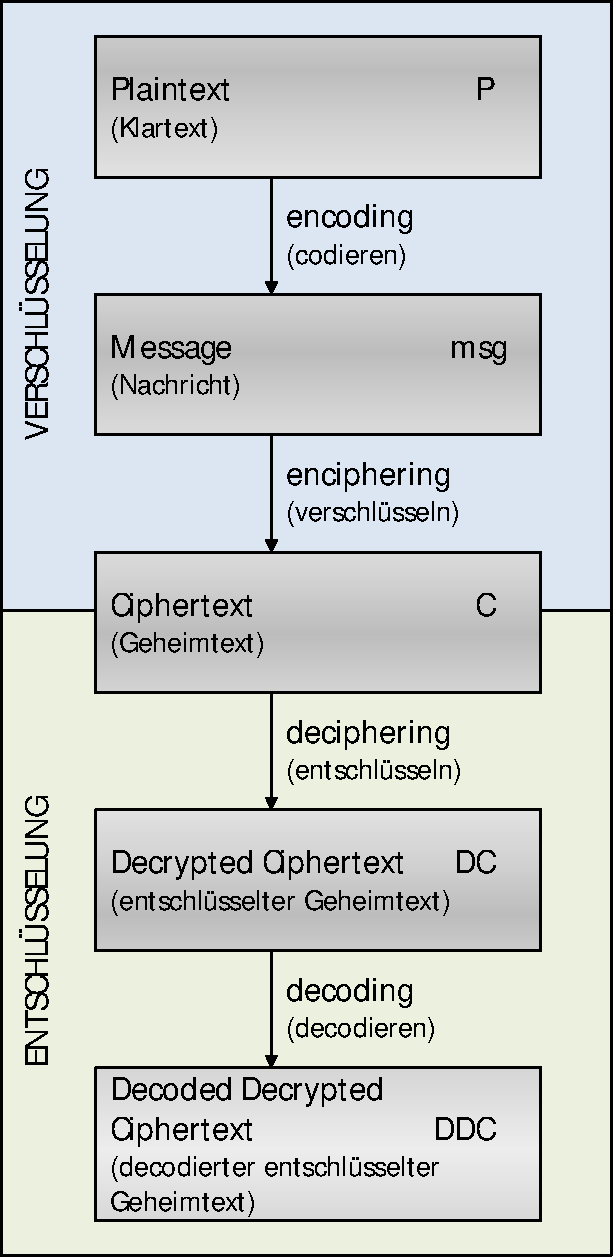
\includegraphics[scale=0.45]{figures/notation-enc-dec_in-sage-scripts_de}
\caption{Namenskonventionen in den SageMath-Programmbeispielen}
\label{naming-convention-in-Sage-cipher-samples}
\end{center}
\end{figure}



% ---------------------------------------------------------------------------
\newpage
\subsection{Transpositions-Chiffren}
\index{Transposition}

Tranpositions-Chiffren sind implementiert in der SageMath-Klasse
\begin{center}
\verb!sage.crypto.classical.TranspositionCryptosystem!
\end{center}
Bevor man mit einer SageMath Transpositions-Chiffre arbeiten kann, muss man sie
konstruieren: Dazu legt man das Alphabet fest, das sie Symbole (Zeichen) enthält,
aus denen Klartext und Geheimtext bestehen können.
Typischerweise besteht das Alphabet aus den normalen lateinischen Großbuchstaben.
Dieses Alphabet legt man mit der folgenden Funktion fest
\begin{center}
\verb!sage.monoids.string_monoid.AlphabeticStrings!
\end{center}
Danach muss man die Blocklänge der Permutation festlegen, d.h. die
Länge des Zeilenvektors der einfachen Spaltentransposition.
Dieser Zeilenvektor ist der Schlüssel, mit dem die Buchstaben des
Klartextes permutiert werden.

Im folgenden ersten Beispiel der Transpositions-Chiffren ist die
Blocklänge 14, und der Schlüssel ist so gebaut, dass jeder Buchstabe
im Klartext um zwei Zeichen nach rechts geshiftet wird (und wrap-around
am Ende des Blocks). Das ist der Verschlüsselungsvorgang.
Der Ent"-schlüsselungsvorgang besteht im Shiften jedes Zeichens des
Geheimtextes um $14 - 2 = 12$ Zeichen nach links.

% Using [fontsize=\footnotesize,fontshape=tt] caused:
%   LaTeX Font Warning: Font shape `T1/cmtt/m/tt' undefined
%   (Font)              using `T1/cmtt/m/n' instead on input line 730.
% so deleted the fontshape parameter.
\begin{sagecode}
\begin{Verbatim}%
[fontsize=\footnotesize]
sage: # transposition cipher using a block length of 14
sage: T = TranspositionCryptosystem(AlphabeticStrings(), 14)
sage: # given plaintext
sage: P   = "a b c d e f g h i j k l m n"
sage: # encryption key
sage: key = [3, 4, 5, 6, 7, 8, 9, 10, 11, 12, 13, 14, 1, 2]
sage:
sage: # encode plaintext (get rid of non-alphabet chars, convert lower-case to upper-case)
sage: msg = T.encoding(P)
sage: # encrypt plaintext by shifting to the left by 2 letters (do it in two steps)
sage: E   = T(key)
sage: C   = E(msg); C
CDEFGHIJKLMNAB
sage:
sage: # decrypt ciphertext by shifting to the left by 12 letters
sage: keyInv = [13, 14, 1, 2, 3, 4, 5, 6, 7, 8, 9, 10, 11, 12]
sage: D   = T(keyInv)
sage: D(C)
ABCDEFGHIJKLMN
sage:
sage: # Representation of key and inverse key as permutations
sage: E
(1,3,5,7,9,11,13)(2,4,6,8,10,12,14)
sage: D
(1,13,11,9,7,5,3)(2,14,12,10,8,6,4)
\end{Verbatim}
\caption{Einfache Transposition durch Shiften (die Schlüssel sind explizit gegeben)}
\end{sagecode}

\newpage
Das zweite Beispiel der Transpositions-Chiffren ist ebenfalls eine einfache
shiftende Spaltentransposition. Aber hier ist der Programmcode ein wenig mehr
automatisiert: Die Schlüssel werden anhand des Shift-Wertes generiert.

\begin{sagecode}
\begin{Verbatim}%
[fontsize=\footnotesize]
sage: # transposition cipher using a block length of 14, code more variable
sage: keylen = 14
sage: shift = 2
sage: A = AlphabeticStrings()
sage: T = TranspositionCryptosystem(A, keylen)
sage:
sage: # construct the plaintext string from the first 14 letters of the alphabet plus blanks
sage: # plaintext   = "A B C D E F G H I J K L M N"
sage: A.gens()
(A, B, C, D, E, F, G, H, I, J, K, L, M, N, O, P, Q, R, S, T, U, V, W, X, Y, Z)
sage: P=''
sage: for i in range(keylen): P=P + " " + str(A.gen(i))
....:
sage: P
' A B C D E F G H I J K L M N'
sage:
sage: # encryption key
sage: # key = [3, 4, 5, 6, 7, 8, 9, 10, 11, 12, 13, 14, 1, 2]
sage: key = [(i+shift).mod(keylen) + 1 for i in range(keylen)]; key
[3, 4, 5, 6, 7, 8, 9, 10, 11, 12, 13, 14, 1, 2]
sage:
sage: # encode plaintext (get rid of non-alphabet chars)
sage: msg = T.encoding(P)
sage: # encrypt plaintext by shifting to the left by 2 letters (do it in one step)
sage: C   = T.enciphering(key, msg); C
CDEFGHIJKLMNAB
sage:
sage: # decrypt ciphertext by shifting to the left by 12 letters
sage: # keyInv = [13, 14, 1, 2, 3, 4, 5, 6, 7, 8, 9, 10, 11, 12]
sage: shiftInv=keylen-shift;
sage: keyInv = [(i+shiftInv).mod(keylen) + 1 for i in range(keylen)]; keyInv
[13, 14, 1, 2, 3, 4, 5, 6, 7, 8, 9, 10, 11, 12]
sage: DC   = T.enciphering(keyInv, C); DC
ABCDEFGHIJKLMN
sage:
sage: # decryption using the "deciphering method with key" instead of "enciphering with keyInv"
sage: # using the deciphering method requires to change the type of the variable key
sage: DC  = T.deciphering(T(key).key(), C); DC
ABCDEFGHIJKLMN
sage:
sage: # representation of key and inverse key as permutations
sage: T(key)
(1,3,5,7,9,11,13)(2,4,6,8,10,12,14)
sage: T(key).key()
(1,3,5,7,9,11,13)(2,4,6,8,10,12,14)
sage: T(keyInv)
(1,13,11,9,7,5,3)(2,14,12,10,8,6,4)
\end{Verbatim}
\caption{Einfache Transposition durch Shiften (die Schlüssel werden mit
         \glqq range\grqq~konstruiert)}
%  ( "`range"' wird in Verzeichnis genauso geschrieben.)
%  ( ``range'' ging auch. )
\end{sagecode}

\newpage
\begin{sloppypar}
Im dritten Beispiel der Transpositions-Chiffren wird eine beliebige Permutation
als Schlüssel für die Ver- und Entschlüsselung gewählt, um die Zeichen in jedem Block
zu verwürfeln (Blocklän"-ge = Anzahl Spalten in der einfachen Spaltentransposition).
Ist die Blocklänge $n$, dann ist der Schlüssel eine Permutation über $n$ Zeichen.
Das folgende Beispiel nutzt die Methode \verb!random_key()! der Klasse
\verb!TranspositionCryptosystem!.  Jeder Aufruf von \verb!random_key()! erzeugt
einen anderen Schlüssel. Deshalb werden bei Ihrem Aufruf voraussichtlich andere
Ergebnisse (Schlüssel und Geheimtext) auftreten.
\end{sloppypar}

\begin{sagecode}
\begin{Verbatim}%
[fontsize=\footnotesize]
sage: # Remark: Enciphering here requires, that the length of msg is a multiple of keylen
sage: keylen = 14   # length of key
sage: A = AlphabeticStrings()
sage: T = TranspositionCryptosystem(A, keylen); T
Transposition cryptosystem on Free alphabetic string monoid on A-Z of block length 14
sage:
sage: P = "a b c d e f g h i j k l m n o p q r s t u v w x y z a b"
sage: key = T.random_key(); key
(1,2,3,13,6,5,4,12,7)(11,14)
sage: msg = T.encoding(P); msg
ABCDEFGHIJKLMNOPQRSTUVWXYZAB
sage: C   = T.enciphering(key, msg); C
BCMLDEAHIJNGFKPQAZRSOVWXBUTY
sage: # decryption using the "deciphering method with key" instead of "enciphering with keyInv"
ssage: DC  = T.deciphering(key, C); DC
ABCDEFGHIJKLMNOPQRSTUVWXYZAB
sage:
sage: # Just another way of decryption: Using "enciphering" with the inverse key
sage: keyInv = T.inverse_key(key); keyInv
(1,7,12,4,5,6,13,3,2)(11,14)
sage: DC     = T.enciphering(keyInv, C); DC
ABCDEFGHIJKLMNOPQRSTUVWXYZAB
sage:
sage: # Test correctness of decryption
sage: msg == DC
True
\end{Verbatim}
\caption{Einfache Spalten-Transposition mit zufällig erzeugtem Schlüssel}
\end{sagecode}


\newpage
Das vierte Beispiel der Transpositions-Chiffren gibt zusätzlich die Größe des Schlüsselraums
einer einfachen Spaltentransposition aus.

\begin{sagecode}
\begin{Verbatim}%
[fontsize=\footnotesize]
sage: keylen = 14   # length of key
sage: A = AlphabeticStrings()
sage: T = TranspositionCryptosystem(A, keylen); T
Transposition cryptosystem on Free alphabetic string monoid on A-Z of block length 14
sage: T.key_space()
Symmetric group of order 14! as a permutation group
sage: # Remark: The key space is not quite correct as also permutations shorter than keylen are counted.
sage:
sage: P = "a b c d e f g h i j k l m n o p q r s t u v w x y z a b"
sage: key = T.random_key(); key
(1,2,7)(3,9)(4,5,10,12,8,13,11)(6,14)
sage: msg = T.encoding(P); msg
ABCDEFGHIJKLMNOPQRSTUVWXYZAB
sage:
sage: # enciphering in one and in two steps
sage: C   = T.enciphering(key, msg); C
BGIEJNAMCLDHKFPUWSXBOAQZRVYT
sage:
sage: enc = T(key); enc.key()
(1,2,7)(3,9)(4,5,10,12,8,13,11)(6,14)
sage: C = enc(msg); C
BGIEJNAMCLDHKFPUWSXBOAQZRVYT
sage:
sage: # deciphering
sage: DC  = T.deciphering(key, C); DC
ABCDEFGHIJKLMNOPQRSTUVWXYZAB
\end{Verbatim}
\caption{Einfache Spalten-Transposition (mit Ausgabe der Größe des Schlüsselraumes)}
\end{sagecode}



% ---------------------------------------------------------------------------
\newpage
\subsection{Substitutions-Chiffren}
\index{Substitution}

Substitutions-Verschlüsselungen sind in SageMath in der folgenden Klasse implementiert
\begin{center}
\verb!sage.crypto.classical.SubstitutionCryptosystem!
\end{center}

\noindent Das folgende Programmbeispiel lässt SageMath eine Substitutions-Chiffre mit
einem zufälligen Schlüssel erstellen. Den zufälligen Schlüssel kann man mit der Methode
\verb!random_key()! der Klasse \texttt{Sub"-stitutionCryptosystem} erzeugen.
Unterschiedliche Schlüssel erzeugen eine unterschiedliche Substitutions-Chiffre.
Deshalb erhält man mit jedem Aufruf von \verb!random_key()! voraussichtlich
ein anderes Ergebnis.

\begin{sagecode}
\begin{Verbatim}%
[fontsize=\footnotesize]
sage: # plaintext/ciphertext alphabet
sage: A   = AlphabeticStrings()
sage: S   = SubstitutionCryptosystem(A)
sage:
sage: P   = "Substitute this with something else better."
sage: key = S.random_key(); key
INZDHFUXJPATQOYLKSWGVECMRB
sage:
sage: # method encoding can be called from A or from T
sage: msg = A.encoding(P); msg
SUBSTITUTETHISWITHSOMETHINGELSEBETTER
sage: C   = S.enciphering(key, msg); C
WVNWGJGVGHGXJWCJGXWYQHGXJOUHTWHNHGGHS
sage:
sage: # We now decrypt the ciphertext to recover our plaintext.
sage:
sage: DC  = S.deciphering(key, C); DC
SUBSTITUTETHISWITHSOMETHINGELSEBETTER
sage: msg == DC
True
\end{Verbatim}
\caption{Monoalphabetische Substitution mit zufällig erzeugtem Schlüssel}
\end{sagecode}



% ---------------------------------------------------------------------------
\newpage
\subsubsection{Caesar-Chiffre}
\index{Caesar}

Das folgende Programmbeispiel erzeugt eine Caesar-Chiffre.

\begin{sagecode}
\begin{Verbatim}%
[fontsize=\footnotesize]
sage: # plaintext/ciphertext alphabet
sage: A = AlphabeticStrings()
sage: P = "Shift the alphabet three positions to the right."
sage:
sage: # construct Caesar cipher
sage: S = SubstitutionCryptosystem(A)
sage: key = A([3, 4, 5, 6, 7, 8, 9, 10, 11, 12, 13, 14, 15, 16, 17, 18, 19, \
....:          20, 21, 22, 23, 24, 25, 0, 1, 2])
sage:
sage: # encrypt message
sage: msg     = A.encoding(P); msg
SHIFTTHEALPHABETTHREEPOSITIONSTOTHERIGHT
sage: encrypt = S(key); encrypt
DEFGHIJKLMNOPQRSTUVWXYZABC
sage: C       = encrypt(msg); C
VKLIWWKHDOSKDEHWWKUHHSRVLWLRQVWRWKHULJKW
sage:
sage: # Next, we recover the plaintext.
sage: # decrypt message
sage: keyInv = A([23, 24, 25, 0, 1, 2, 3, 4, 5, 6, 7, 8, 9, 10, 11, 12, 13, \
....:             14, 15, 16, 17, 18, 19, 20, 21, 22])
sage: decrypt = S(keyInv); decrypt
XYZABCDEFGHIJKLMNOPQRSTUVW
sage: DC      = decrypt(C); DC
SHIFTTHEALPHABETTHREEPOSITIONSTOTHERIGHT
sage: msg == DC
True
\end{Verbatim}
\caption{Caesar (Substitution durch Shiften des Alphabets; Schlüssel explizit gegeben; Schritt-für-Schritt-Ansatz)}
\end{sagecode}


\newpage
Das zweite Caesar-Beispiel macht dasselbe, aber der Programmcode ist variabler.

\begin{sagecode}
\begin{Verbatim}%
[fontsize=\footnotesize]
sage: # plaintext/ciphertext alphabet
sage: A = AlphabeticStrings()
sage: keylen = len(A.gens()); keylen
26
sage: shift  = 3
sage: P = "Shift the alphabet three positions to the right."
sage:
sage: # construct Caesar cipher
sage: S = SubstitutionCryptosystem(A)
sage: S
Substitution cryptosystem on Free alphabetic string monoid on A-Z
sage: # key = A([3, 4, 5, 6, 7, 8, 9, 10, 11, 12, 13, 14, 15, 16, 17, 18, 19, \
sage: #          20, 21, 22, 23, 24, 25, 0, 1, 2])
sage: key = [(i+shift).mod(keylen) for i in range(keylen)];
sage: key = A(key); key
DEFGHIJKLMNOPQRSTUVWXYZABC
sage: len(key)
26
sage:
sage: # encrypt message
sage: msg     = A.encoding(P); msg
SHIFTTHEALPHABETTHREEPOSITIONSTOTHERIGHT
sage: C       = S.enciphering(key, msg); C
VKLIWWKHDOSKDEHWWKUHHSRVLWLRQVWRWKHULJKW
sage:
sage: # Next, we recover the plaintext.
sage: # decrypt message
sage: # keyInv = A([23, 24, 25, 0, 1, 2, 3, 4, 5, 6, 7, 8, 9, 10, 11, 12, 13, \
sage: #             14, 15, 16, 17, 18, 19, 20, 21, 22])
sage: shiftInv=keylen-shift;
sage: keyInv = [(i+shiftInv).mod(keylen) for i in range(keylen)];
sage: keyInv = A(keyInv); keyInv
XYZABCDEFGHIJKLMNOPQRSTUVW
sage: DC     = S.enciphering(keyInv, C); DC
SHIFTTHEALPHABETTHREEPOSITIONSTOTHERIGHT
sage:
sage: # Just another way of decryption: Using "deciphering" with the key
sage: DC     = S.deciphering(key, C); DC
SHIFTTHEALPHABETTHREEPOSITIONSTOTHERIGHT
sage:
sage: msg == DC
True
\end{Verbatim}
\caption{Caesar (Substitution durch Shiften des Alphabets; Substitutions-Schlüssel wird berechnet)}
\end{sagecode}


% ---------------------------------------------------------------------------
\newpage
\subsubsection{Verschiebe-Chiffre}
\index{Verschiebechiffre}

Die Verschiebe-Chiffre kann man sich auch als Verallgemeinerung der ursprünglichen
Caesar-Chiffre denken: Caesar shiftete das Alphabet immer genau um 3 Positionen.
Die Shift-Chiffre kann um eine beliebige Anzahl Positionen entlang des
Alphabets shiften. Shiften ist eine spezielle Form der Substitution.

In den obigen Beispielen wurde das \verb!SubstitutionCryptosystem! angewandt, und
Caesar wurde als Sonderfall der Substitution implementiert. Andererseits
kann man Caesar auch Spezialfall der Shift-Chiffre betrachten.

Die Shift-Chiffre  ist direkt implementiert in der SageMath-Klasse
\begin{center}
\verb!sage.crypto.classical.ShiftCryptosystem!
\end{center}

Im folgenden Beispiel konstruieren wir eine Shift-Chiffre über den Großbuchstaben
des lateinischen Alphabets. Dann verschlüsseln wir den Klartext P durch Shiften
um 12 Positionen. Schließlich entschlüsseln wir wieder das Chiffrat C und überprüfen,
dass das Ergebnis (DC) identisch mit dem ursprünglichen Klartext ist.

\begin{sagecode}
\begin{Verbatim}%
[fontsize=\footnotesize]
sage: # construct Shift cipher directly
sage: shiftcipher = ShiftCryptosystem(AlphabeticStrings()); shiftcipher
Shift cryptosystem on Free alphabetic string monoid on A-Z
sage: P = shiftcipher.encoding("Shift me any number of positions."); P
SHIFTMEANYNUMBEROFPOSITIONS
sage: key = 12  # shift can be any integer number
sage: # shift the plaintext by 12 positions to get the ciphertext
sage: C = shiftcipher.enciphering(key, P); C
ETURFYQMZKZGYNQDARBAEUFUAZE
sage:
sage: # decrypt the ciphertext and ensure that it is the original plaintext
sage: DC = shiftcipher.deciphering(key, C); DC
SHIFTMEANYNUMBEROFPOSITIONS
sage: DC == P
True
\end{Verbatim}
\caption{Verschiebe-Chiffre (über dem Großbuchstabenalphabet)}
\label{paper_pencil:shift_cipher:Sage_example}
\end{sagecode}

Die ursprüngliche Caesar-Chiffre ist eine Shift-Chiffre mit
festem Schlüssel 3. Im nächsten Beispiel wird die Caesar-Chiffre
über den Großbuchstaben des lateinischen Alphabets gebaut.
% Dann verschlüsseln wir den
% Klartext P mit der Caesar-Chiffre. Schließlich entschlüsseln wir
% wieder das Chiffrat C und überprüfen, dass das Ergebnis (DC)
% identisch mit dem ursprünglichen Klartext ist.

\begin{sagecode}
\begin{Verbatim}%
[fontsize=\footnotesize]
sage: caesarcipher = ShiftCryptosystem(AlphabeticStrings())
sage: P = caesarcipher.encoding("Shift the alphabet by three positions to the right."); P
SHIFTTHEALPHABETBYTHREEPOSITIONSTOTHERIGHT
sage:
sage: key = 3  # shift the plaintext by exactly 3 positions
sage: C = caesarcipher.enciphering(key, P); C
VKLIWWKHDOSKDEHWEBWKUHHSRVLWLRQVWRWKHULJKW
sage:
sage: # decrypt the ciphertext and ensure that it is the original plaintext
sage: DC = caesarcipher.deciphering(key, C); DC
SHIFTTHEALPHABETBYTHREEPOSITIONSTOTHERIGHT
sage: DC == P
True
\end{Verbatim}
\caption{Caesar-Verschlüsselung mit der Verschiebe-Chiffre}
\label{paper_pencil:shift_cipher:Sage_example_Caesar_cipher}
\end{sagecode}


% ---------------------------------------------------------------------------
\newpage
\subsubsection{Affine Chiffren}
\label{PaP_affine_cipher_sage-sample}
\index{affine Chiffre}

Die affine Chiffre ist implementiert in der SageMath-Klasse
\begin{center}
\verb!sage.crypto.classical.AffineCryptosystem!
\end{center}

Im folgenden Beispiel konstruieren wir eine affine Chiffre $ c_i = b*p_i + a $
mit dem Schlüssel $(3, 13)$ und benutzen sie, um einen gegebenen Klartext
$P = (p_1,p_2, ...,p_n)$ zu verschlüsseln. Der Klartext wird dann wieder
entschlüsselt und das Ergebnis DC mit dem ursprünglichen Klartext verglichen.

\begin{sagecode}
\begin{Verbatim}%
[fontsize=\footnotesize]
sage: # create an affine cipher
sage: affineCipher = AffineCryptosystem(AlphabeticStrings()); affineCipher
Affine cryptosystem on Free alphabetic string monoid on A-Z
sage: P = affineCipher.encoding("The affine cryptosystem.")
sage: P
THEAFFINECRYPTOSYSTEM
sage:
sage: # encrypt the plaintext using the key (3, 13)
sage: a, b = (3, 13)
sage: C = affineCipher.enciphering(a, b, P)
sage: C
SIZNCCLAZTMHGSDPHPSZX
sage:
sage: # decrypt the ciphertext and make sure that it is equivalent to the original plaintext
sage: DC = affineCipher.deciphering(a, b, C)
sage: DC
THEAFFINECRYPTOSYSTEM
sage: DC == P
True
\end{Verbatim}
\caption{Affine Chiffre mit dem Schlüssel $(3, 13)$}
\end{sagecode}


Man kann  die Shift-Chiffre auch als Sonderfall der affinen Chiffre sehen.
Dazu muss man den Schlüssel der affinen Chiffre auf die folgende Form
$(1, b)$ einschränken, wobei $b$ jede ganze, nicht-negative Zahl sein kann.
Das SageMath-Beispiel~\ref{paper_pencil:shift_cipher:Sage_example} auf
Seite~\pageref{paper_pencil:shift_cipher:Sage_example} kann man
wie folgt darstellen:

\begin{sagecode}[h]
\begin{Verbatim}%
[fontsize=\footnotesize]
sage: # construct a shift cipher
sage: shiftcipher = AffineCryptosystem(AlphabeticStrings()); shiftcipher
Affine cryptosystem on Free alphabetic string monoid on A-Z
sage: P = shiftcipher.encoding("Shift me any number of positions.")
sage: P
SHIFTMEANYNUMBEROFPOSITIONS
sage:
sage: # shift the plaintext by 12 positions to get the ciphertext
sage: a, b = (1, 12)
sage: C = shiftcipher.enciphering(a, b, P)
sage: C
ETURFYQMZKZGYNQDARBAEUFUAZE
sage:
sage: # decrypt the ciphertext and ensure that it is the original plaintext
sage: DC = shiftcipher.deciphering(a, b, C); P
SHIFTMEANYNUMBEROFPOSITIONS
sage: DC == P
True
\end{Verbatim}
\caption{Verschiebe-Chiffre (als Sonderfall der affinen Chiffre)}
\end{sagecode}


Man kann mit der affinen Chiffre auch eine Caesar-Chiffre bauen. Dazu muss
der Ver-/Entschlüsselungsschlüssel den Wert $(1, 3)$ haben.
Das SageMath-Beispiel~\ref{paper_pencil:shift_cipher:Sage_example_Caesar_cipher}
auf Seite~\pageref{paper_pencil:shift_cipher:Sage_example_Caesar_cipher}
kann mit der affinen Chiffre folgendermaßen dargestellt werden.

\begin{sagecode}
\begin{Verbatim}%
[fontsize=\footnotesize]
sage: # create a Caesar cipher
sage: caesarcipher = AffineCryptosystem(AlphabeticStrings())
sage: P = caesarcipher.encoding("Shift the alphabet by three positions to the right.")
sage: P
SHIFTTHEALPHABETBYTHREEPOSITIONSTOTHERIGHT
sage:
sage: # shift the plaintext by 3 positions
sage: a, b = (1, 3)
sage: C = caesarcipher.enciphering(a, b, P)
sage: C
VKLIWWKHDOSKDEHWEBWKUHHSRVLWLRQVWRWKHULJKW
sage:
sage: # decrypt the ciphertext and ensure that it is the original plaintext
sage: DC = caesarcipher.deciphering(a, b, C)
sage: DC
SHIFTTHEALPHABETBYTHREEPOSITIONSTOTHERIGHT
sage: DC == P
True
\end{Verbatim}
\caption{Caesar-Chiffre (als Sonderfall der affinen Chiffre)}
\end{sagecode}



% ---------------------------------------------------------------------------
\newpage
\subsubsection{Substitutions-Chiffre mit Symbolen}
\index{Substitution}

Im folgenden SageMath-Programmbeispiel sind die Alphabetzeichen aus dem Binärsystem.
Eine monoalphabetische Substitution über einem Binäralphabet bietet nur wenig
Sicherheit: Weil das Klartext-/Geheimtext-Alphabet nur aus den 2 Elementen
0 und 1 besteht, gibt es nur zwei mögliche Schlüssel: (0 1) und (1 0). \\
Anmerkung: Im Schlüssel einer allgemeinen Substitutions-Chiffre müssen
alle Alphabetzeichen genau einmal auftreten.

\begin{sagecode}
\begin{Verbatim}%
[fontsize=\footnotesize]
sage: # the plaintext/ciphertext alphabet
sage: B = BinaryStrings()
sage: # substitution cipher over the alphabet B; no keylen argument possible
sage: S = SubstitutionCryptosystem(B); S
Substitution cryptosystem on Free binary string monoid
sage: # To get a substitute for each symbol, key has always the length of the alphabet
sage: key = S.random_key(); key
10
sage: len(key)
2
sage: P = "Working with binary numbers."
sage: # encryption
sage: msg = B.encoding(P); msg
01010111011011110111001001101011011010010110111001100111001000000111011101101\
00101110100011010000010000001100010011010010110111001100001011100100111100100\
1000000110111001110101011011010110001001100101011100100111001100101110
sage: C   = S.enciphering(key, msg); C
10101000100100001000110110010100100101101001000110011000110111111000100010010\
11010001011100101111101111110011101100101101001000110011110100011011000011011\
0111111001000110001010100100101001110110011010100011011000110011010001
sage: # decryption
sage: DC  = S.deciphering(key, C); DC
01010111011011110111001001101011011010010110111001100111001000000111011101101\
00101110100011010000010000001100010011010010110111001100001011100100111100100\
1000000110111001110101011011010110001001100101011100100111001100101110
sage: msg == DC
True
\end{Verbatim}
\caption{Monoalphabetische Substitution über dem Binär-Alphabet}
\end{sagecode}

Anmerkung: Im Moment hat \verb!S! kein Attribut \verb!key!, und ich fand
keine Möglichkeit, den Binärstring \verb!DC! wieder in ASCII zurück zu verwandeln.


\newpage
\begin{sloppypar}
Das zweite Beispiel einer monoalphabetischen Substitution mit Symbolen benutzt
ein größeres Alphabet für den Klartext-/Geheimtext-Zeichenraum als das erste Beispiel.
Hier wird nun das hexadezimale Zahlensystem als Substitutions-Alphabet verwendet.
\end{sloppypar}

\begin{sagecode}
\begin{Verbatim}%
[fontsize=\footnotesize]
sage: A = HexadecimalStrings()
sage: S = SubstitutionCryptosystem(A)
sage: key = S.random_key(); key
2b56a4e701c98df3
sage: len(key)
16
sage: # Number of possible keys
sage: factorial(len(key))
20922789888000
sage: P   = "Working with a larger alphabet."
sage:
sage: msg = A.encoding(P); msg
576f726b696e6720776974682061206c617267657220616c7068616265742e
sage: C   = S.enciphering(key, msg); C
47e375e9e1efe75277e17ae052eb52e8eb75e7e47552ebe872e0ebe5e47a5f
sage: DC  = S.deciphering(key, C); DC
576f726b696e6720776974682061206c617267657220616c7068616265742e
sage: msg == DC
True
sage:
sage: # Conversion hex back to ASCII:
sage: # - AlphabeticStrings() and HexadecimalStrings() don't have according methods.
sage: # - So we used Python directly.
sage: import binascii
sage: DDC = binascii.a2b_hex(repr(DC)); DDC
'Working with a larger alphabet.'
sage:
sage: P == DDC
True
\end{Verbatim}
\caption{Monoalphabetische Substitution über dem Hexadezimal-Alphabet (Dekodieren in Python\index{Python})}
\end{sagecode}



% ---------------------------------------------------------------------------
\newpage
\subsubsection{Vigen{\`e}re-Verschlüsselung}
\index{Vigen\`ere}

Die Vigen{\`e}re-Verschlüsselung ist in der folgenden SageMath-Klasse implementiert
\begin{center}
\verb!sage.crypto.classical.VigenereCryptosystem!
\end{center}

\noindent Als Klartext-/Geheimtext-Zeichenraum kann man die lateinischen
Großbuchstaben, das Binär"-system, das Oktalsystem oder Hexadezimalsystem wählen.
Hier ist ein Beispiel, das mit der Klasse \verb!AlphabeticStrings! die Großbuchstaben
nutzt.

\begin{sagecode}
\begin{Verbatim}%
[fontsize=\footnotesize]
sage: # construct Vigenere cipher
sage: keylen = 14
sage: A = AlphabeticStrings()
sage: V = VigenereCryptosystem(A, keylen); V
Vigenere cryptosystem on Free alphabetic string monoid on A-Z of period 14
sage:
sage: # alternative could be a given key: key = A('ABCDEFGHIJKLMN'); key
sage: key = V.random_key(); key
WSSSEEGVVAARUD
sage: len(key)
14
sage:
sage: # encoding
sage: P = "The Vigenere cipher is polyalphabetic."
sage: len(P)
38
sage: msg = V.encoding(P); msg     # alternative: msg = A.encoding(P); msg
THEVIGENERECIPHERISPOLYALPHABETIC
sage:
sage: # encryption [2 alternative ways (in two steps or in one): both work]
sage: # encrypt = V(key); encrypt
sage: # C = encrypt(msg); C
sage: C   = V.enciphering(key, msg); C
PZWNMKKIZRETCSDWJAWTUGTALGBDXWLAG
sage:
sage: # decryption
sage: DC  = V.deciphering(key, C); DC
THEVIGENERECIPHERISPOLYALPHABETIC
sage: msg == DC
True
\end{Verbatim}
\caption{Vigen{\`e}re-Verschlüsselung}
\end{sagecode}




% ---------------------------------------------------------------------------
\newpage
\subsection{Hill-Verschlüsselung}
\index{Hill}

Die Hill~\cite{Hill1929,Hill1931}- oder Matrix-Verschlüsselung\footnote{%
   In CT1\index{CT1} kann man dieses Verfahren über den Menüeintrag
   \textbf{Ver-/Entschlüsseln \textbackslash{} Symmetrisch (klassisch)
   \textbackslash{} Hill} aufrufen.\\
   In CT2\index{CT2} findet sich dieses Verfahren bei den Vorlagen
   unter \textbf{Kryptographie \textbackslash{} Klassisch} und
   unter \textbf{Kryptoanalyse \textbackslash{} Klassisch}.
   }
ist mathematisch anspruchsvoller als die Verfahren in den bisherigen
Programmbeispielen dieses Kapitels. Der Schlüssel dieses
Verfahrens ist eine invertierbare quadratische Matrix (hier $key$ genannt).
Klartext und Geheimtext sind Vektoren ($P$ und $C$).
Die Ver- und Entschlüsselungsprozesse nutzen Matrizen-Operationen modulo 26,
hier also $C = P * key$ $(mod$ $26)$.

\noindent Die Hill-Verschlüsselung ist implementiert in der SageMath-Klasse
\begin{center}
\verb!sage.crypto.classical.HillCryptosystem!
\end{center}

\noindent Im folgenden Beispiel besteht der Klar-/Geheimtext-Zeichenraum wieder
aus den Großbuchstaben des lateinischen Alphabets. Im Hill-Verfahren wird
jedem Alphabet-Zeichen eine eindeutige natürliche Zahl modulo 26 zugewiesen.
Die Größe der Schlüssel-Matrix (auch Matrix-Dimension genannt) ist vom
Hill-Verfahren selbst nicht beschränkt.\\

\noindent \textbf{Bemerkung:} Vergleich der Hill-Implementierung in
CrypTool v1.4.31 und in SageMath Version 5.3:
\begin{itemize}
  \item SageMath bietet schnelle Operationen auf der Kommandozeile;
        CT1 stellt seine Funktionalität nur in einer GUI zur Verfügung.
  \item SageMath bietet für die Schlüssel-Matrix jede Matrix-Dimension an;
        CT1 ist beschränkt auf die Werte 1 bis 10.
  \item SageMath erlaubt auch negative Zahlen in der Schlüssel-Matrix
        und konvertiert diese selbststän"-dig in nicht-negative Werte;
        CT1 erlaubt keine negativen Zahlen in der Schlüssel-Matrix.
  \item SageMath weist dem ersten Alphabet-Zeichen immer den Wert 0 zu;\\
        SageMath lässt hierbei nur die 26 Großbuchstaben als Alphabet zu;\\
        und es nutzt nur die Multiplikationsvariante
        Klartext-Zeilenvektor * Schlüsselmatrix:\\
        $C = P * key$.
  \item CT1 erlaubt die Wahl zwischen 0 und 1 für das erste
        Alphabet-Zeichen; man kann sein Alphabet im Textoptionen-Dialog
        zusammen stellen; und es bietet auch die umgekehrte
        Multiplikationsvariante: $C = key * P$
\end{itemize}

\begin{figure}[ht]
\begin{center}
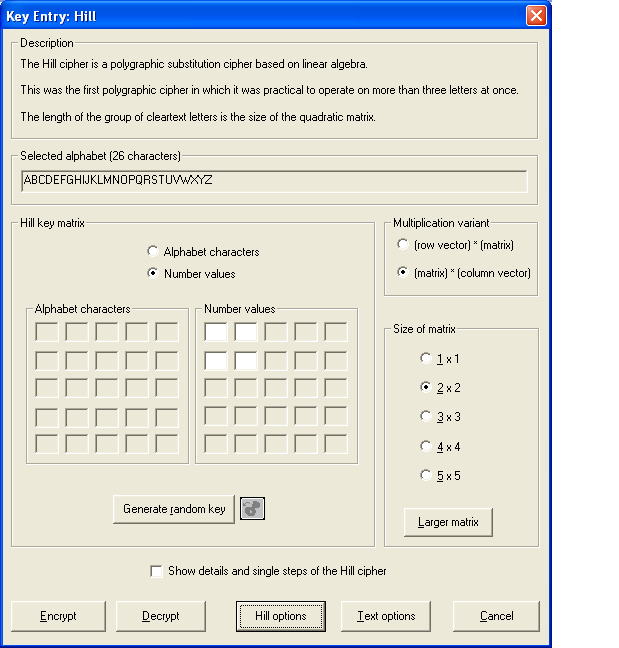
\includegraphics[scale=0.7]{figures/PaP_Fig_Hill-Cipher-CT-Dialog.png}
\caption{Hill-Dialog in CT1 mit den verfügbaren Operationen und Optionen\vspace{1ex}}
\label{PaP_Fig_Hill-Cipher-CT-Dialog}
\end{center}
\end{figure}

\begin{sagecode}
\begin{Verbatim}%
[fontsize=\footnotesize]
sage: # construct a Hill cipher
sage: keylen = 19    # An Alternative could be: Use a non-random small key (e.g. keylen = 3)
sage: A = AlphabeticStrings(); H = HillCryptosystem(A, keylen); H
Hill cryptosystem on Free alphabetic string monoid on A-Z of block length 19
sage:
sage: # Alternative: Here, HKS is necessary in addition [H.key_space() isn't enough].
sage: # HKS = H.key_space(); key = HKS([[1,0,1],[0,1,1],[2,2,3]]); key
sage:
sage: # Random key creation
sage: key = H.random_key(); key
[10  7  5  2  0  6 10 23 15  7 17 19 18  2  9 12  0 10 11]
[23  1  1 10  4  9 21  1 25 22 19  8 17 22 15  8 12 25 22]
[ 4 12 16 15  1 12 24  5  9 13  5 15  8 21 23 24 22 20  6]
[ 5 11  6  7  3 12  8  9 21 20  9  4 16 18 10  3  2 23 18]
[ 8 22 14 14 20 13 21 19  3 13  2 11 13 23  9 25 25  6  8]
[24 25  8 24  7 18  3 20  6 11 25  5  6 19  7 24  2  4 10]
[15 25 11  1  4  7 11 24 20  2 18  4  9  8 12 19 24  0 12]
[14  6  2  9 11 20 13  4 10 11  4 23 14 22 14 16  9 12 18]
[12 10 21  5 21 15 16 17 19 20  1  1 15  5  0  2 23  4 14]
[21 15 15 16 15 20  4 10 25  7 15  4  7 12 24  9 19 10  6]
[25 15  2  3 17 23 21 16  8 18 23  4 22 11 15 19  6  0 15]
[14 23  9  3 18 15 10 18  7  5 12 23 11  9 22 21 20  4 14]
[ 3  6  8 13 20 16 11  1 13 10  4 21 25 15 12  3  0 11 18]
[21 25 14  6 11  3 21  0 19 17  5  8  5  4  9  2 23 19 15]
[ 8 11  9 11 20 15  6  1  3 18 18 22 16 17  6  3 15 11  2]
[21 15  5 22  2  9  0  4 22 10  2 10 19 19 17 19  1 21  4]
[ 7 17  9  2 15  5 14  3  6  9 12 12 22 15  8  4 21 14 19]
[19 14 24 19  7  5 22 22 13 14  7 18 17 19 25  2  1 23  6]
[ 2  6 14 22 17  7 23  6 22  7 13 20  0 14 23 17  6  1 12]
sage:
sage: # encoding and encryption
sage: P = "Hill or matrix cipher uses matrix operations."; len(P)
45
sage: # implementation requires: Length of msg is a multiple of matrix dimension (block_length)
sage: msg = H.encoding(P); msg; len(msg)
HILLORMATRIXCIPHERUSESMATRIXOPERATIONS
38
sage:
sage: # encryption (the length of msg must be a multiple of keylen).
sage: C  = H.enciphering(key, msg); C
CRWCKPRVYXNBRZTNZCTQWFWSDWBCHABGMNEHVP
sage:
sage: # decryption
sage: DC  = H.deciphering(key, C); DC; msg == DC
HILLORMATRIXCIPHERUSESMATRIXOPERATIONS
True
sage:
sage: # alternative decryption using inverse matrix
sage: keyInv = H.inverse_key(key); keyInv
[ 6 23  1 23  3 12 17 22  6 16 22 14 18  3  1 10 21 16 20]
[18 23 15 25 24 23  7  4 10  7 21  7  9  0 13 22  5  5 23]
...
[10 11 12  6 11 17 13  9 19 16 14 24  4  8  5 16 18 20  1]
[19 16 16 21  1 19  7 12  3 18  1 17  7 10 24 21  7 16 11]
sage: DC     = H.enciphering(keyInv, C); DC
HILLORMATRIXCIPHERUSESMATRIXOPERATIONS
\end{Verbatim}
\caption{Hill-Verschlüsselung mit einer zufällig generierten Schlüsselmatrix}
\end{sagecode}

%------------------------------------------------------------------------------

\printbibliography[%
	heading=subbibintoc,
	title={Literatur zu Kapitel \thechapter},
	segment=\therefsegment,
]


\noindent Alle Links wurden am 11.07.2016 überprüft.

\end{refsegment}

% Local Variables:
% TeX-master: "../script-de.tex"
% End:

